\documentclass[12pt,a4paper]{article}
\usepackage[T1]{fontenc}
\usepackage[polish]{babel}
\usepackage{geometry}
\usepackage{fancyhdr}
\usepackage{graphicx}
\usepackage{booktabs}
\usepackage{float}
\usepackage{hyperref}

\geometry{margin=2.5cm}

\title{Projekt MPUM - Raport}
\author{Jakub Trela \and Karol Bielaszka}
\date{}

\pagestyle{fancy}
\fancyhf{}
\rhead{MPUM Projekt}
\lhead{Raport}
\cfoot{\thepage}

\begin{document}
\maketitle

\section*{Wstęp}
W ramach naszego projektu pracujemy na zbiorze danych \href{https://www.kaggle.com/datasets/irkaal/foodcom-recipes-and-reviews}{Food.com Recipes and Reviews} dostępnym w serwisie Kaggle. Zawiera on przepisy kulinarne składające się z opisu dania, spisu składników, instrukcji przygotowania, wartości odżywczych (w tym liczby kalorii, tłuszczów, węglowodanów i białek), a także liczby porcji. 

W naszych modelach jako cechy (argumenty wejściowe) rozważamy przede wszystkim same instrukcje przygotowania potrawy, jednak przetestujemy również warianty modeli rozszerzone o dodatkową cechę, jaką jest liczba porcji. Analizując instrukcje tekstowe, pomijamy wartości liczbowe, rozważamy wyłącznie słowa występujące w tekście. Zadaniem modeli jest predykcja liczby kalorii, tłuszczów, węglowodanów oraz białek. 

Z uwagi na specyfikę problemu, gdzie dla modelu sformułowania typu „5g masła” oraz „100g masła” będą zinterpretowane dokładnie tak samo, nie spodziewamy się ekstremalnie wysokich wyników metryk jakościowych. Można jednak założyć, że część istotnych informacji uda się wywnioskować, ponieważ przepisy zamieszczane w Internecie są na ogół przygotowywane dla skończonej i powtarzalnej liczby osób (najczęściej 2--4). Z tego względu rozbieżność w rzeczywistych masach składników nie powinna być drastycznie wielka.

\section*{Analiza danych}
W tej sekcji przedstawiono wstępną analizę struktury oraz statystyk opisowych zbioru danych. Analizie poddano przede wszystkim rozkłady zmiennych objaśnianych (kalorii oraz poszczególnych makroskładników) pod kątem występowania wartości odstających, a także zbadano korelację między długością instrukcji przygotowania a złożonością odżywczą potraw. Dokonano również oczyszczenia tekstu poprzez usunięcie znaków interpunkcyjnych, konwersję na małe litery oraz eliminację tokenów numerycznych.

\section*{Założenia odnośnie modeli}
Do treningu modeli wykorzystujemy zbiór składający się z $120\,000 - \epsilon$ wierszy, gdzie wartość $\epsilon$ wynika z procesu odfiltrowania niepoprawnych lub brakujących cech. Do testów rezerwujemy osobny podzbiór liczący $80\,000 - \epsilon$ wierszy. Przed podziałem dane zostały w pełni przetasowane. 

Do generowania wykresów (zarówno krzywych uczenia, jak i analizy wpływu maksymalnej liczby cech wyekstrahowanych z tekstu) wykorzystujemy zbiór o wielkości $60\,000 - \epsilon$ wierszy, z którego 20\% wydzielamy jako zbiór walidacyjny. Krzywe uczenia obliczamy odpowiednio wartościach około (5\%, 19\%, 32\%, 46\%, 59\% 72\%, 86\%, 100\%) rozwarzanych danych, a krzywe ilości cech na wartościach (10, 50, 100, 300, 600, 1000, 1500, 2000, 4000) cech. Do wektoryzacji tekstu wykorzystujemy metodę TF-IDF – zarówno w wersji z biblioteki \texttt{scikit-learn}, jak i w ramach własnej implementacji. Wstępne testy wykazały, że podejście to radzi sobie znacznie lepiej niż alternatywne metody reprezentacji tekstowej. Rozważamy również wariant „manual TF-IDF”. Główną metryką, na podstawie której oceniamy i porównujemy dopasowanie modeli, jest współczynnik determinacji $R^2$.

\section*{Rozważane modele}

\subsection*{Dumb regressor}
W pierwszej kolejności rozważyliśmy model referencyjny, który zawsze zwraca wartość średnią z danych treningowych. Pozwali ocenić realny zysk z zastosowania bardziej zaawansowanych algorytmów.

\begin{figure}[H]
    \centering
    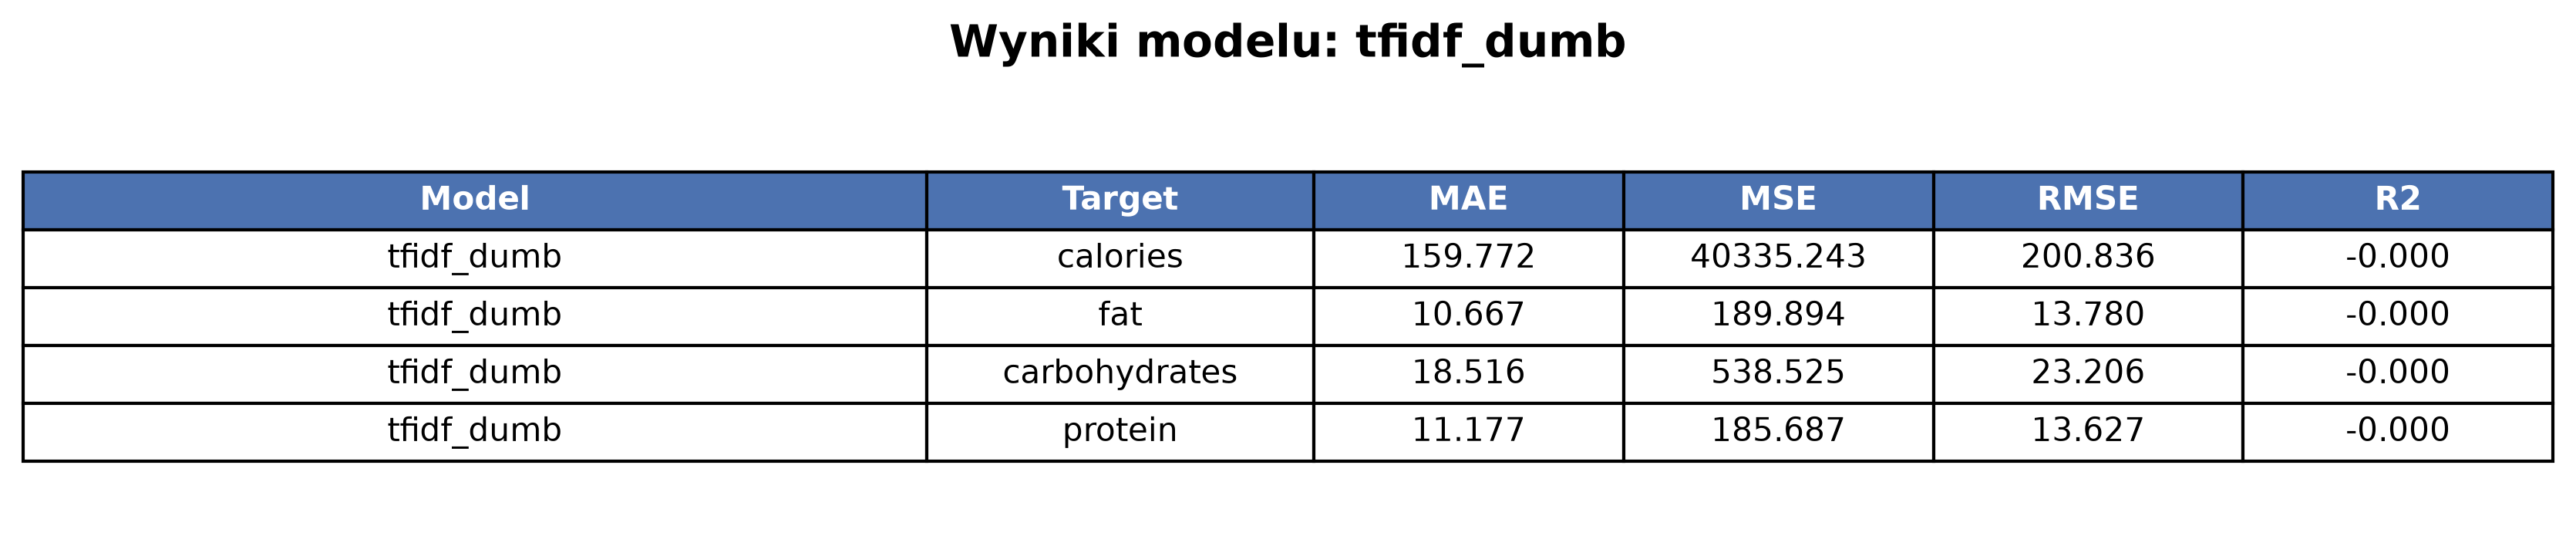
\includegraphics[width=0.8\textwidth]{../img/stats/tfidf_dumb.png}
    %\caption{Statystyki i wyniki predykcji dla modelu referencyjnego (Dumb Regressor).}
    \label{fig:tfidf_dumb}
\end{figure}

Widzimy jak wyglądają błędy i dokładność $R^2$, która szczególnie będzie nas intersować. 

\subsection*{Elastic net gradient descent regressor}
Pierwszym naszym modelem jest regresja liniowa z regularyzacją Elastic Net, zaimplementowana przy pomocy algorytmu stochastycznego spadku gradientu. Z racji nieróżniczkowalności składnika $L_1$ w punkcie zero, w implementacji zastosowaliśmy technikę \textit{soft thresholding}. Jeżeli nasz model przestaje się uczyć, wprowadziliśmy mechanizm dynamicznego zmniejszania współczynnika uczenia (\textit{learning rate}) w celu precyzyjniejszego zlokalizowania minimum globalnego. Jeśli pomimo tego zabiegu wynik na zbiorze walidacyjnym nie ulega poprawie, proces uczenia jest przerywany.

\begin{figure}[H]
    \centering
    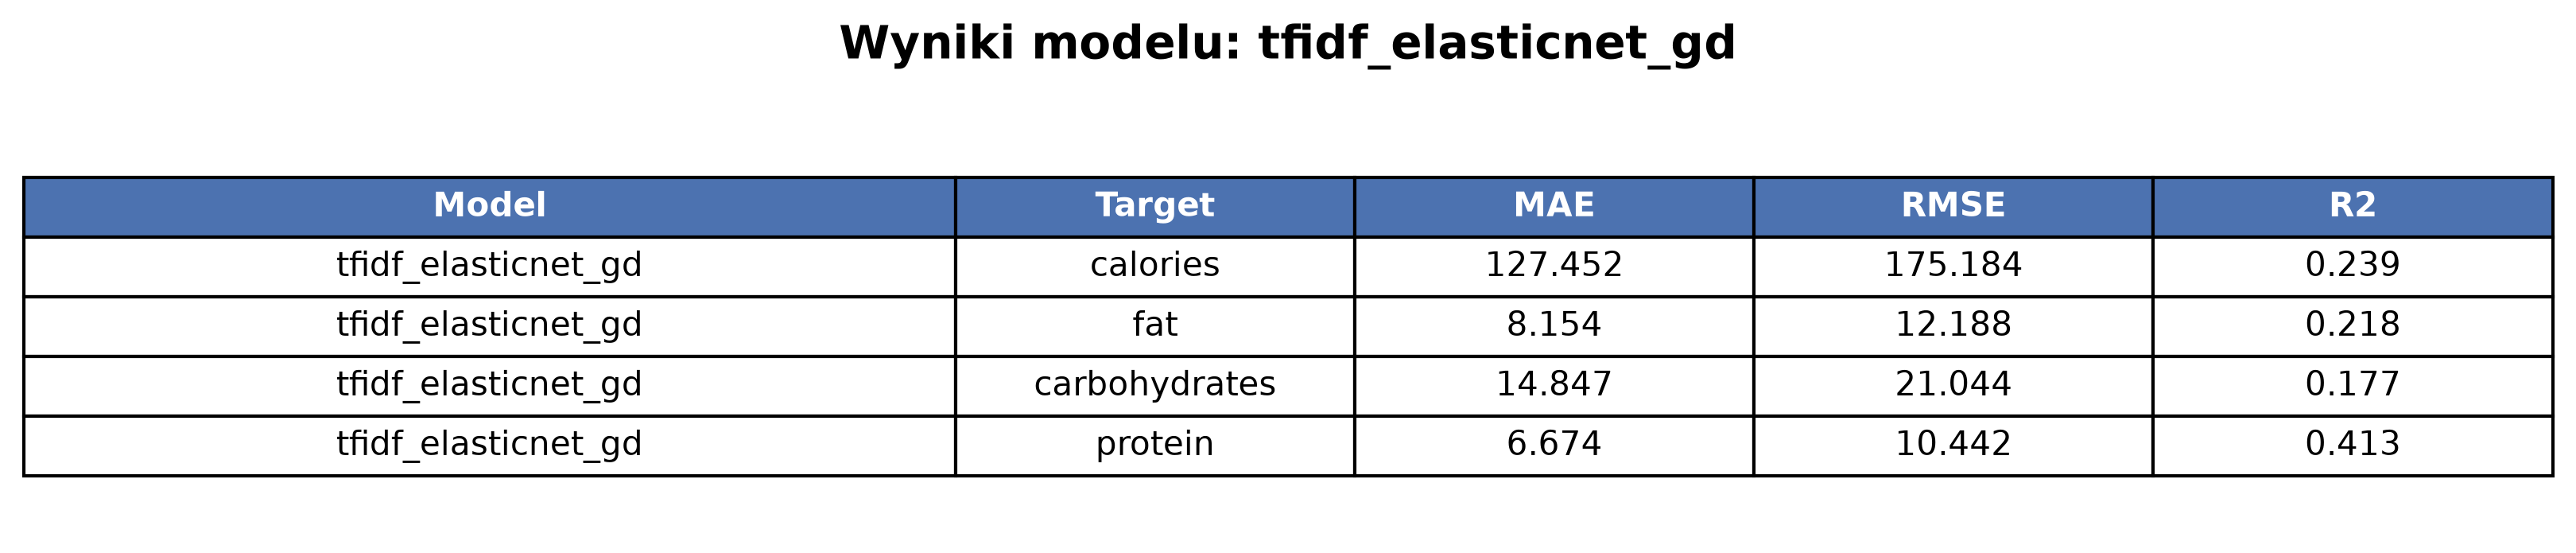
\includegraphics[width=0.8\textwidth]{../img/stats/tfidf_elasticnet_gd.png}
    \vspace{0.5cm}
    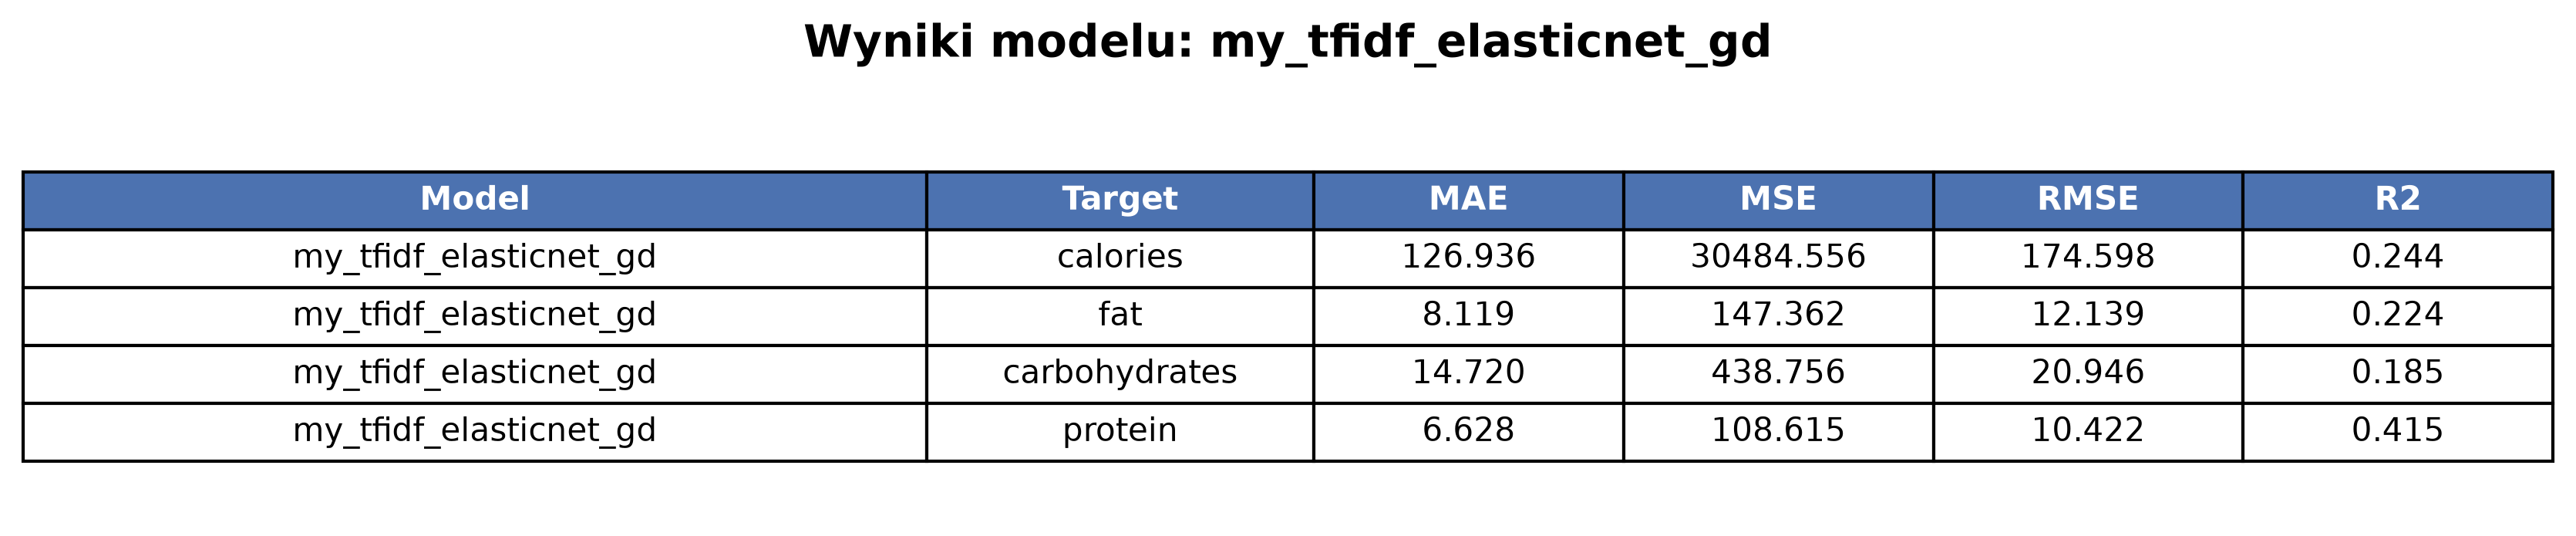
\includegraphics[width=0.8\textwidth]{../img/stats/my_tfidf_elasticnet_gd.png}
    %\caption{Porównanie wyników modelu Elastic Net GD: wersja z biblioteki scikit-learn (góra) oraz własna implementacja (dół).}
    \label{fig:elasticnet_gd_comparison}
\end{figure}

Widzimy, że model działą dość dobrze jak na problem z jakim się mierzymy. Na naszym tfidf otrzymujemy nieco lepsze wyniki.

\begin{figure}[H]
    \centering
    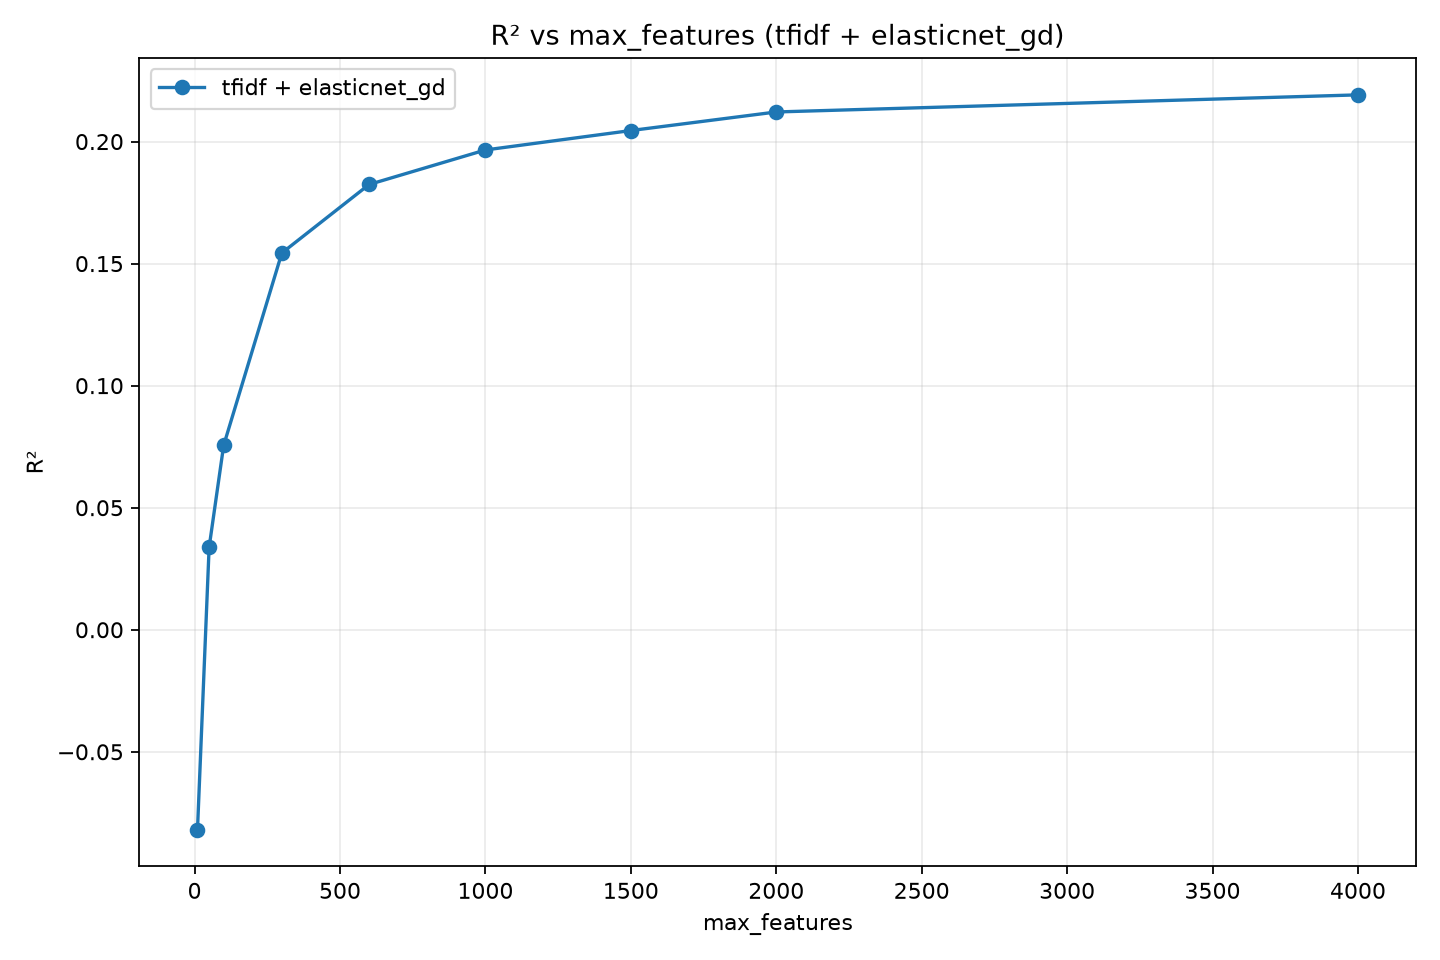
\includegraphics[width=0.48\textwidth]{../img/max_features_tfidf_elasticnet_gd.png}
    %\caption{Wpływ maksymalnej liczby cech (max features) na jakość predykcji modelu Elastic Net GD.}
    \label{fig:max_features_elasticnet}
\end{figure}

Zależność od ilości cech wybranych z tekstu wygląda dość spodziewanie. W praktyce musimy wybrać tylko kilka najważnijszych słów aby określić kalorycznosć.

\subsection*{Ridge}
Dla porównania efektywności optymalizacji gradientowej wykorzystaliśmy model regresji grzbietowej z biblioteki \texttt{scikit-learn}.

\begin{figure}[H]
    \centering
    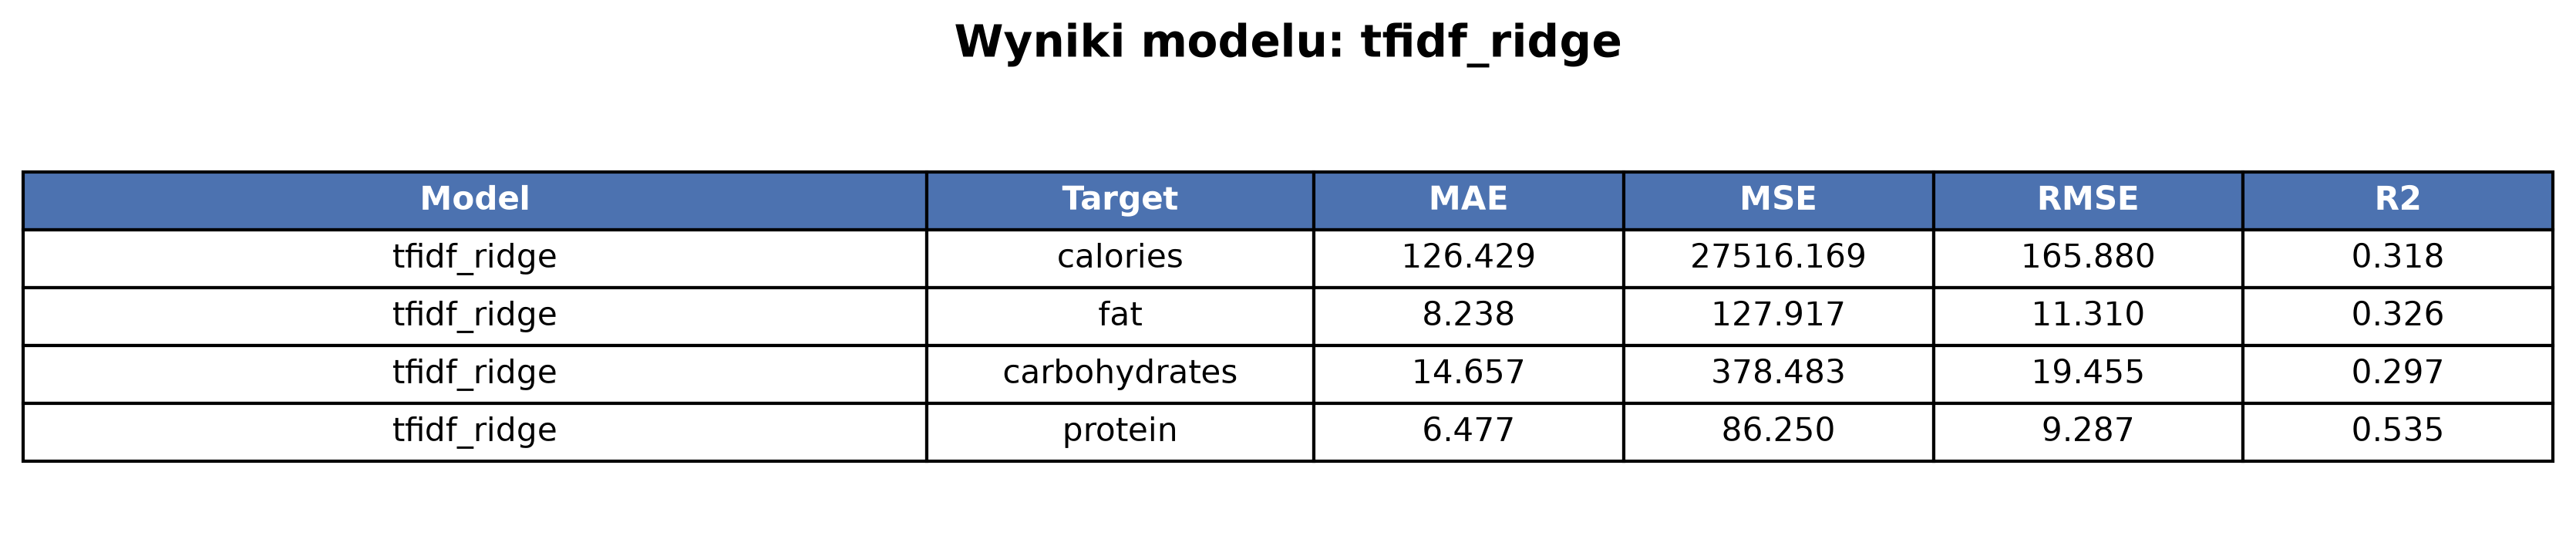
\includegraphics[width=0.8\textwidth]{../img/stats/tfidf_ridge.png}
    \vspace{0.5cm}
    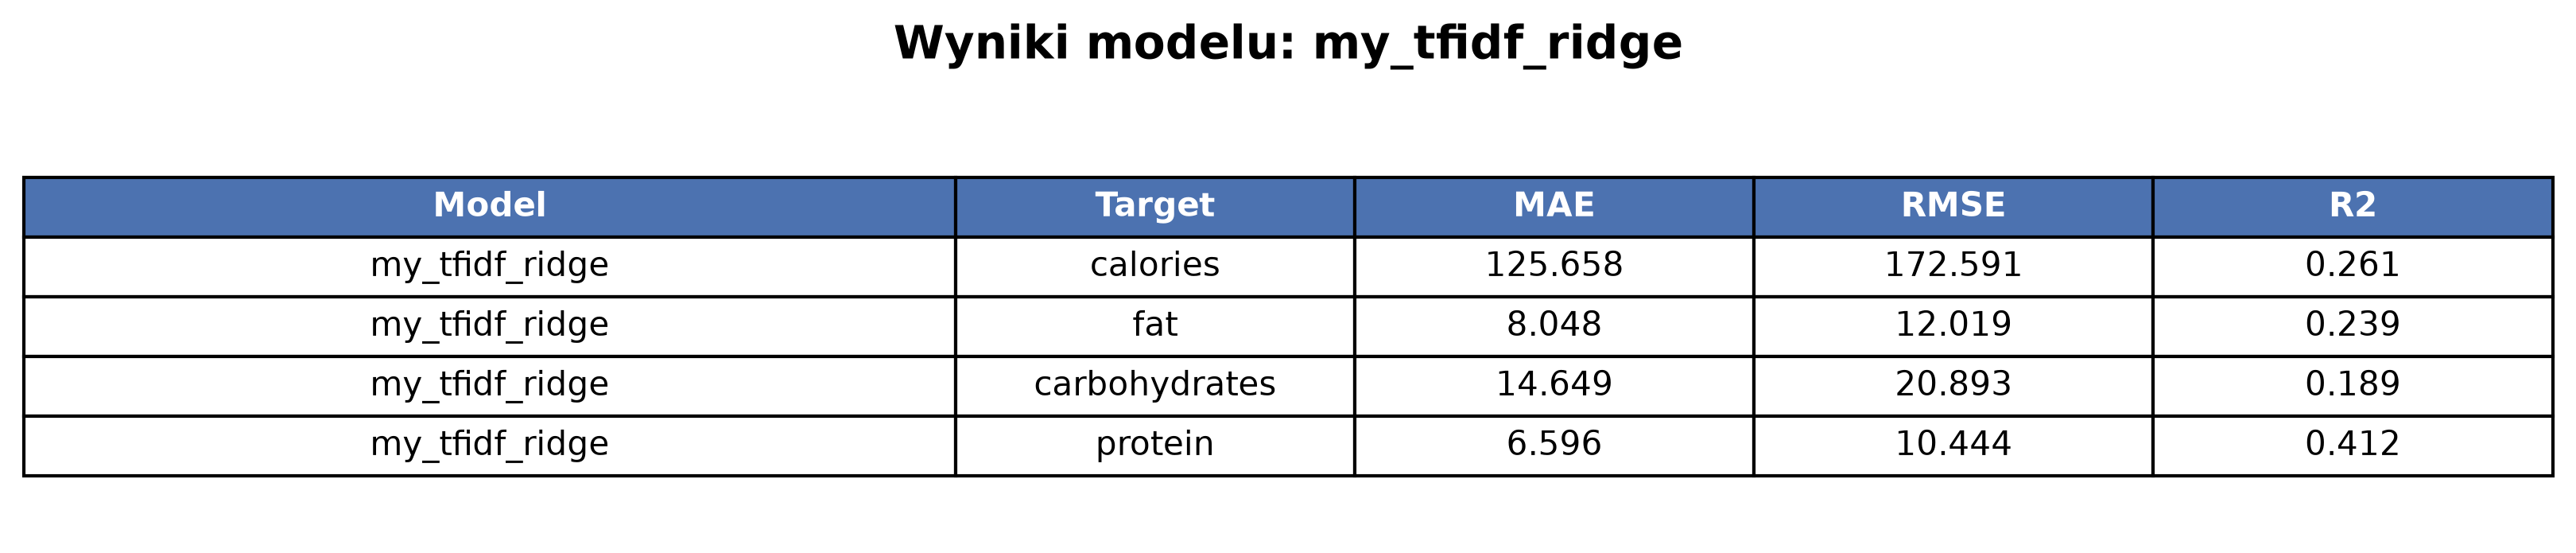
\includegraphics[width=0.8\textwidth]{../img/stats/my_tfidf_ridge.png}
    %\caption{Wyniki dla modelu Ridge Regression: wersja z biblioteki scikit-learn (góra) oraz własna implementacja (dół).}
    \label{fig:ridge_comparison}
\end{figure}

% \begin{figure}[H]
%     \centering
%     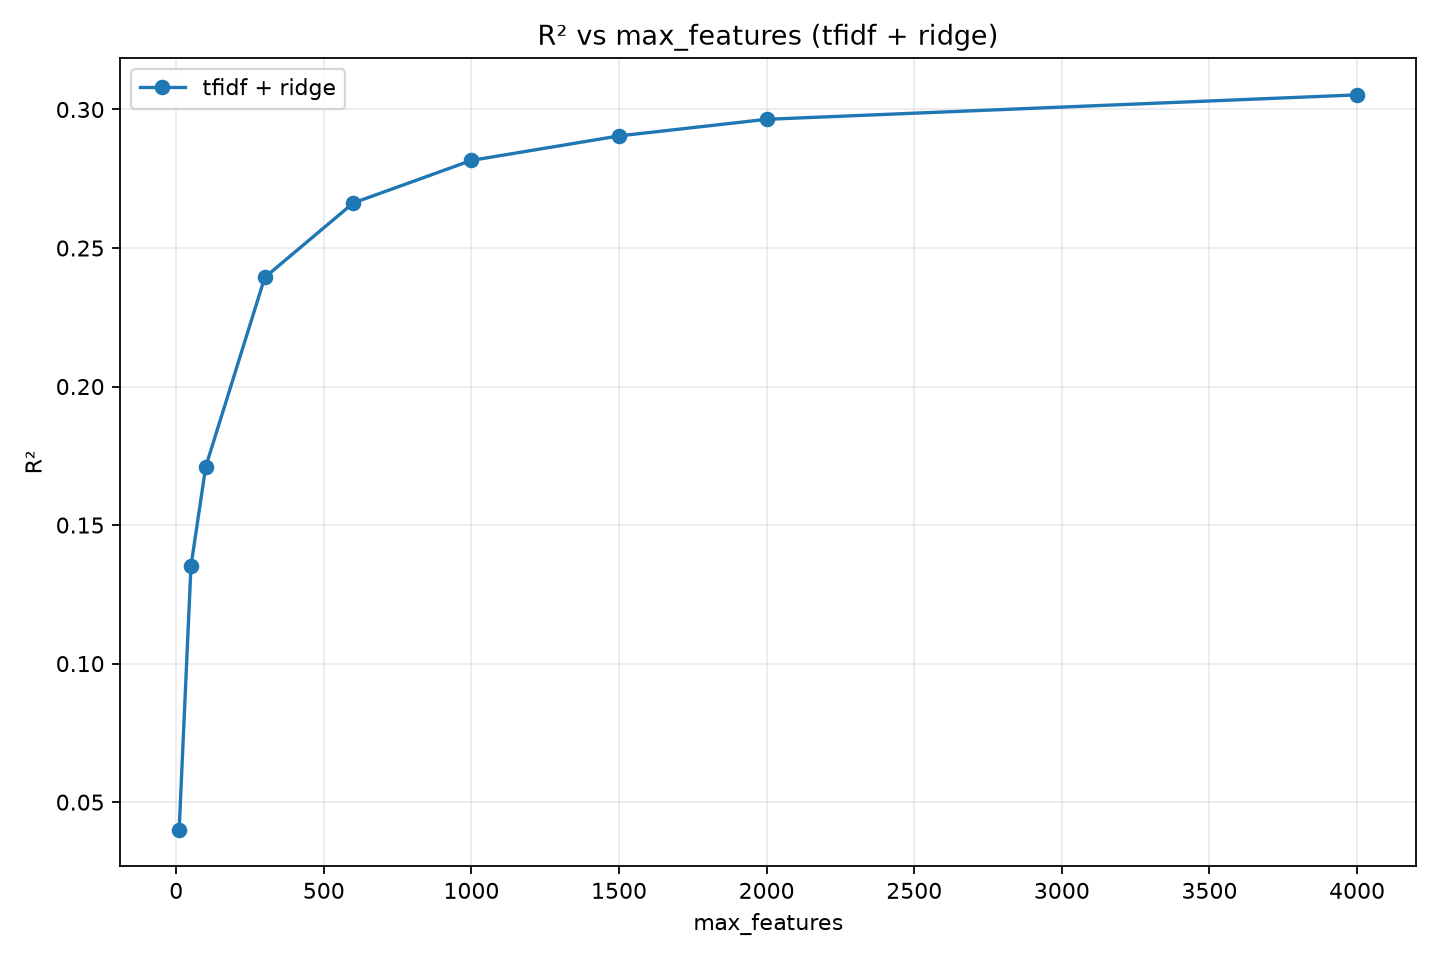
\includegraphics[width=0.48\textwidth]{../img/max_features_tfidf_ridge.png}
%     %\caption{Wpływ maksymalnej liczby cech na współczynnik $R^2$ w modelu Ridge.}
%     \label{fig:max_features_ridge}
% \end{figure}

\begin{figure}[H]
    \centering
    \begin{minipage}{0.48\textwidth}
        \centering
        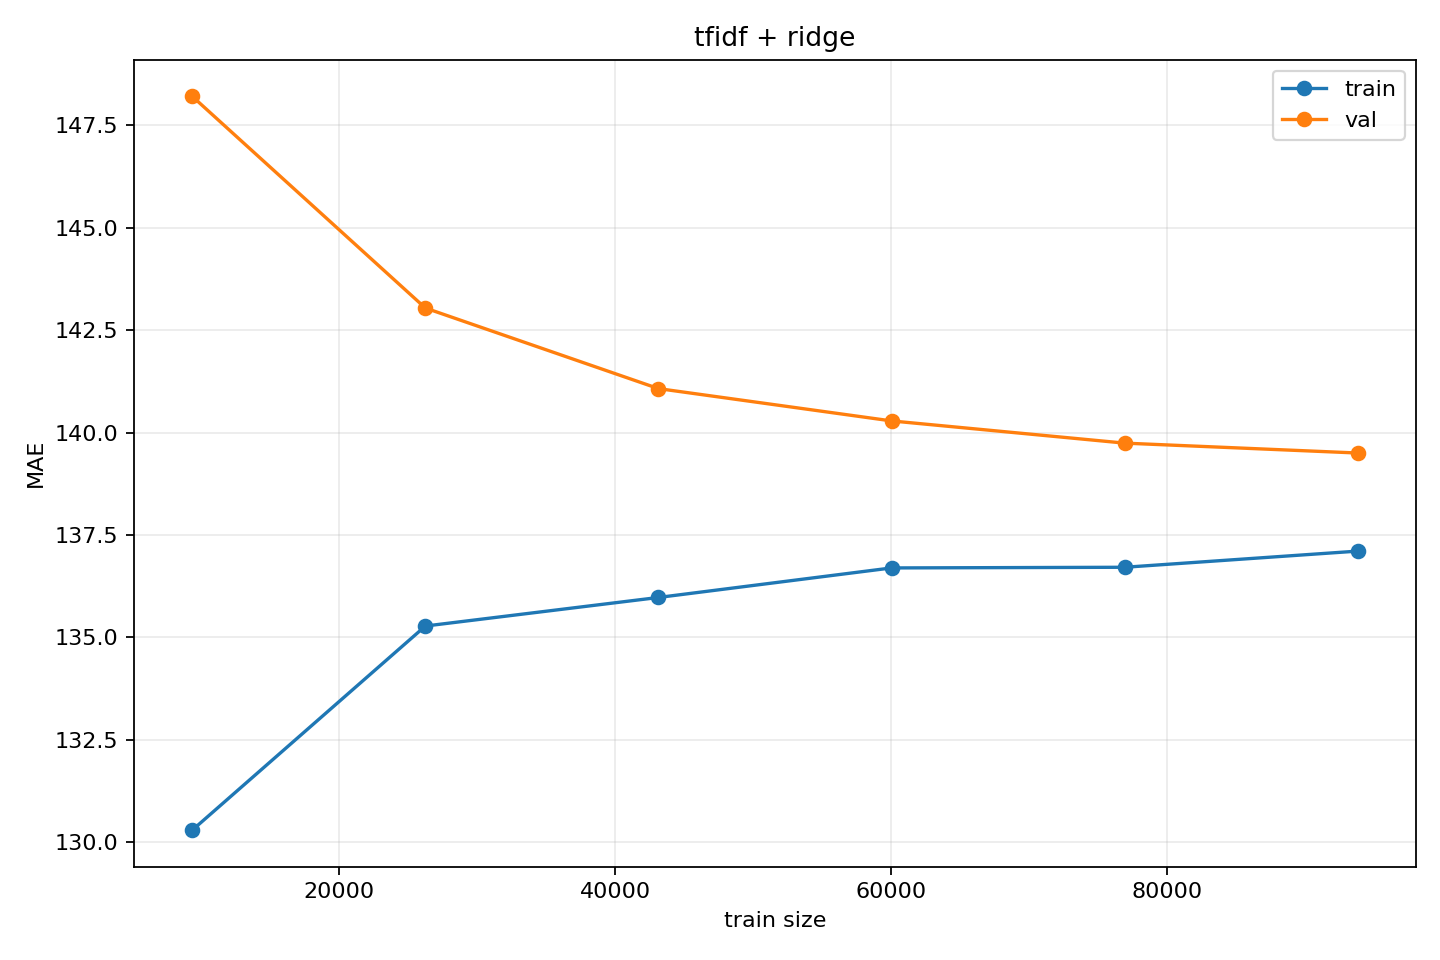
\includegraphics[width=\textwidth]{../img/learning_curve_tfidf__ridge.png}
        \label{fig:learning_curve_nn}
    \end{minipage}
    \hfill
    \begin{minipage}{0.48\textwidth}
        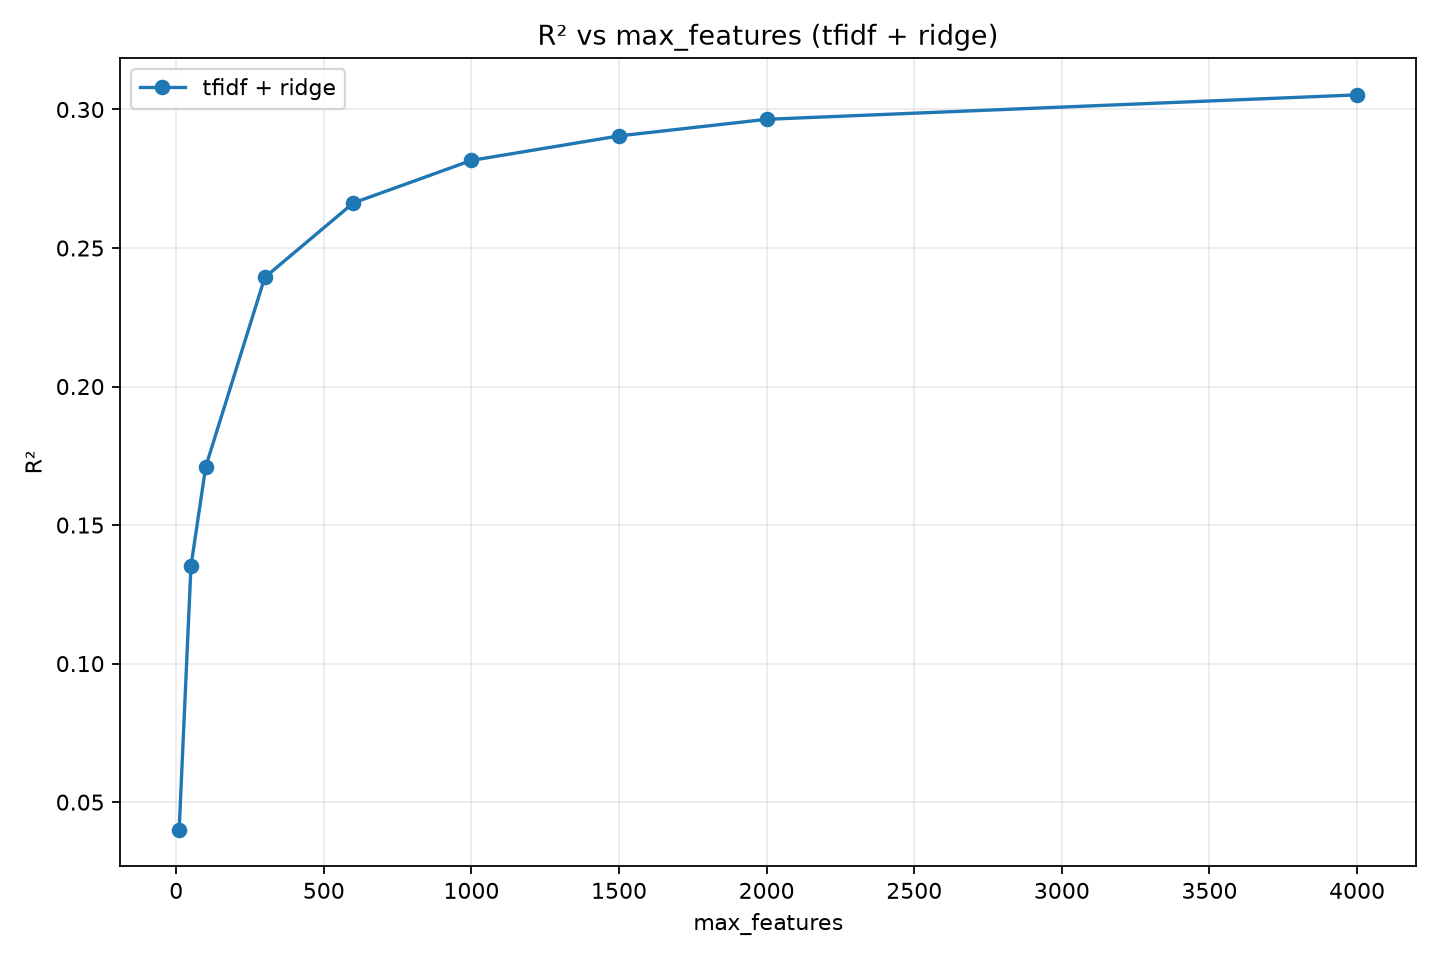
\includegraphics[width=\textwidth]{../img/max_features_tfidf_ridge.png}
        \centering
        \label{fig:max_features_nn}
    \end{minipage}
\end{figure}

Widizmy, że model ze scikit pordzaił sobie lepiej jednak, gorzej współpracuje z naszym wektoryzerm. Krzywa zależność ilości cech wygląda niemal identycznie. Natomiast krzywa uczenia na zbiorze treningowym bardzo łatwo się przeucza, jednak dośc szybko  

Zaimplementowaliśmy również modele bazujący na ręcznie przygotowanym wektorze cech (manual TF-IDF), oraz uwzględniające dodatkowo informację o liczbie porcji, co miało na celu zmniejszenie błędu wynikającego ze skalowalności przepisów.

\begin{figure}[H]
    \centering
    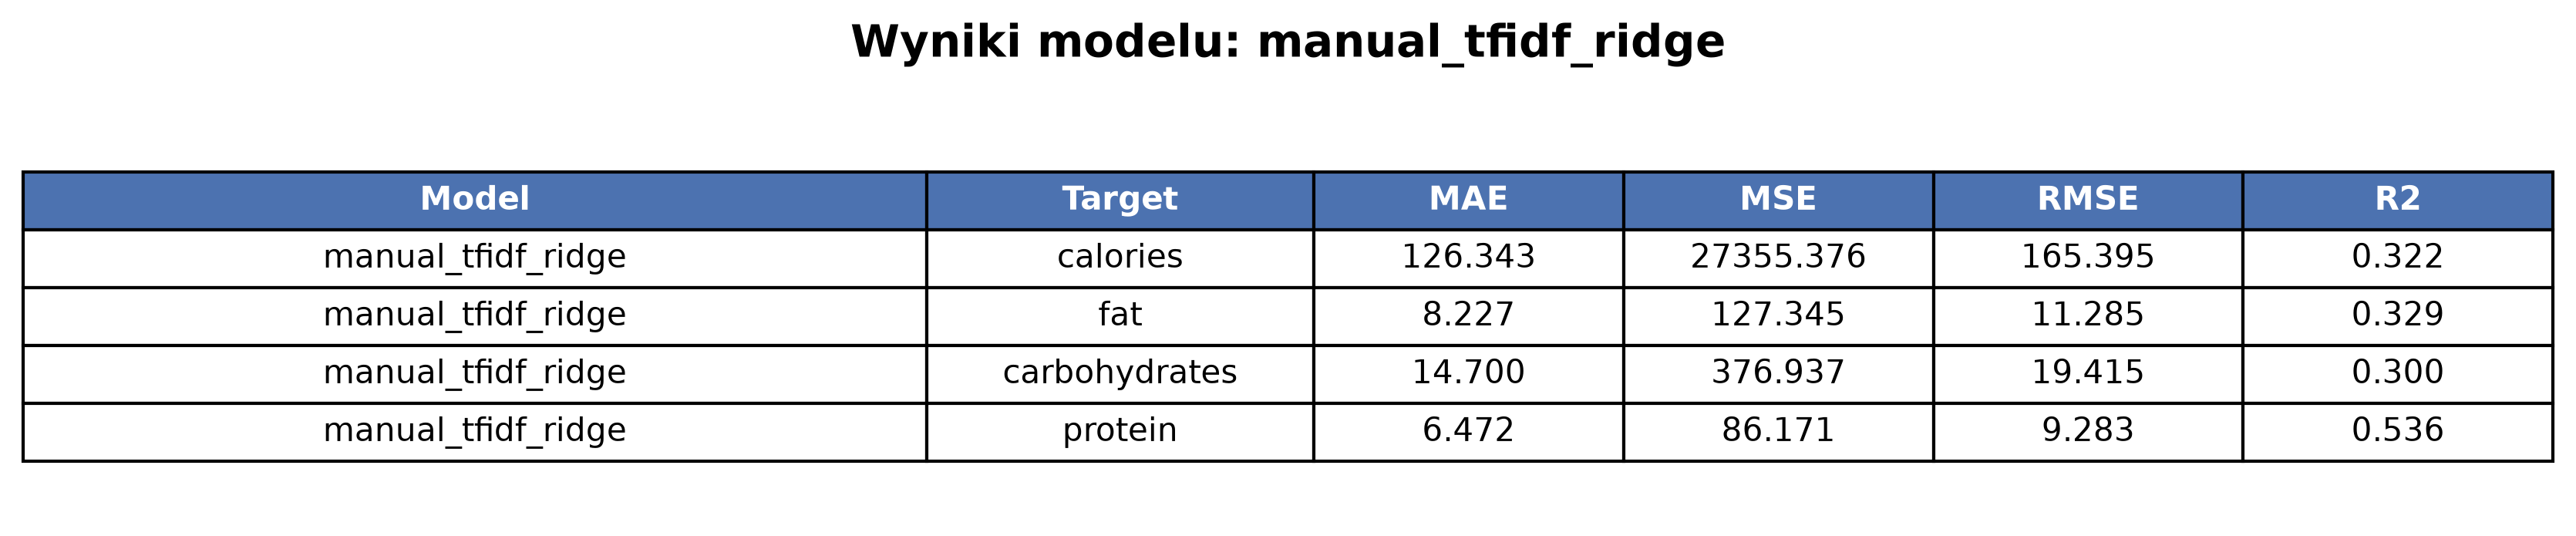
\includegraphics[width=0.8\textwidth]{../img/stats/manual_tfidf_ridge.png}
    \vspace{0.5cm}
    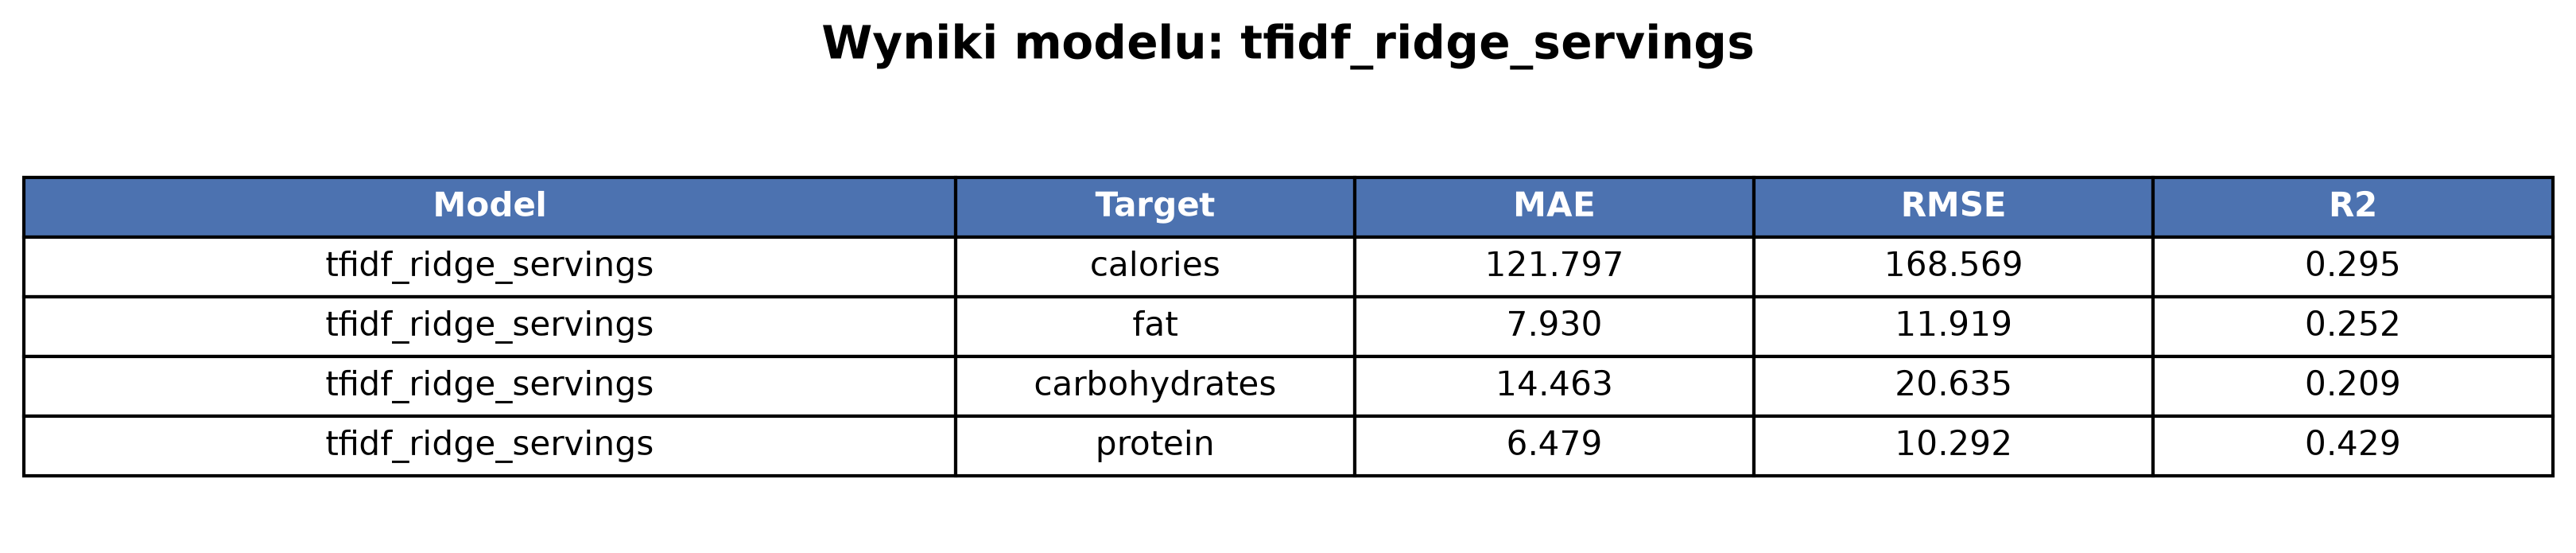
\includegraphics[width=0.8\textwidth]{../img/stats/tfidf_ridge_servings.png}
    \vspace{0.5cm}
    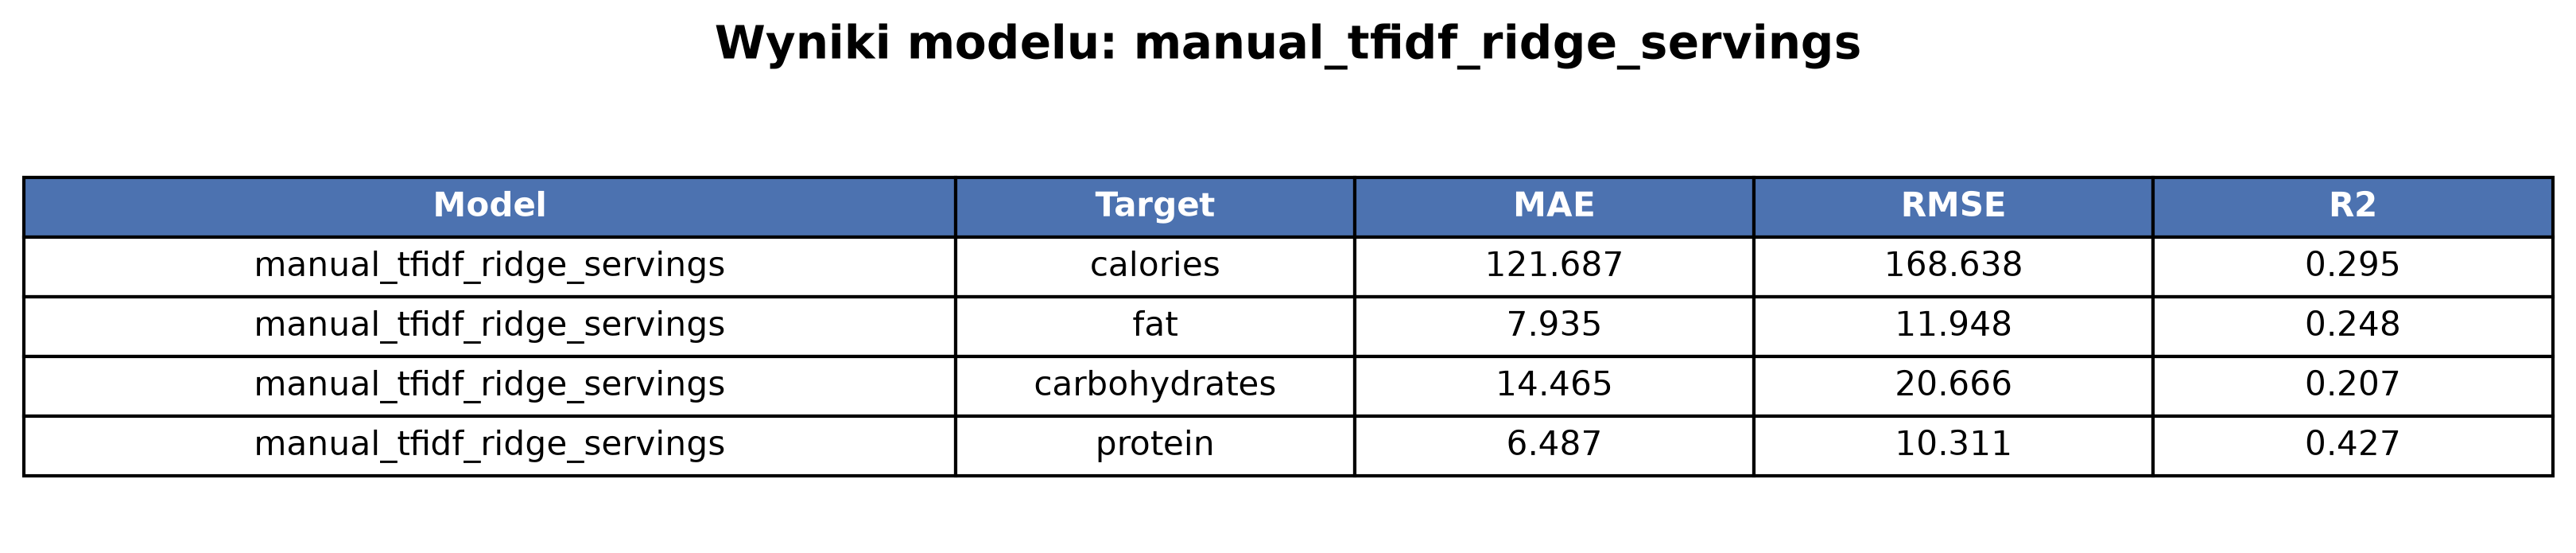
\includegraphics[width=0.8\textwidth]{../img/stats/manual_tfidf_ridge_servings.png}
    \label{fig:manual_tfidf_ridge}
\end{figure}

Możemy zauważyć, że dodanie manualnych cech poprawia model, jednak ilość porcji osłabia.

\subsection*{Neural net}
Kolejnym rozważanym przez nas rozwiązaniem jest sieć neuronowa. Biorąc pod uwagę specyfikę oraz charakter zadania, struktura sieci nie musi być nadmiernie głęboka. Zdecydowaliśmy się na architekturę o dwóch warstwach ukrytych o wielkościach odpowiednio 64 i 32 neurony z funkcjami aktywacji ReLU. Model trenowaliśmy przez 20 epok z learning rate 0.1 oraz batchami wielkości 64. Parametry wdobraliśmy eksperymentalnie.

\begin{figure}[H]
    \centering
    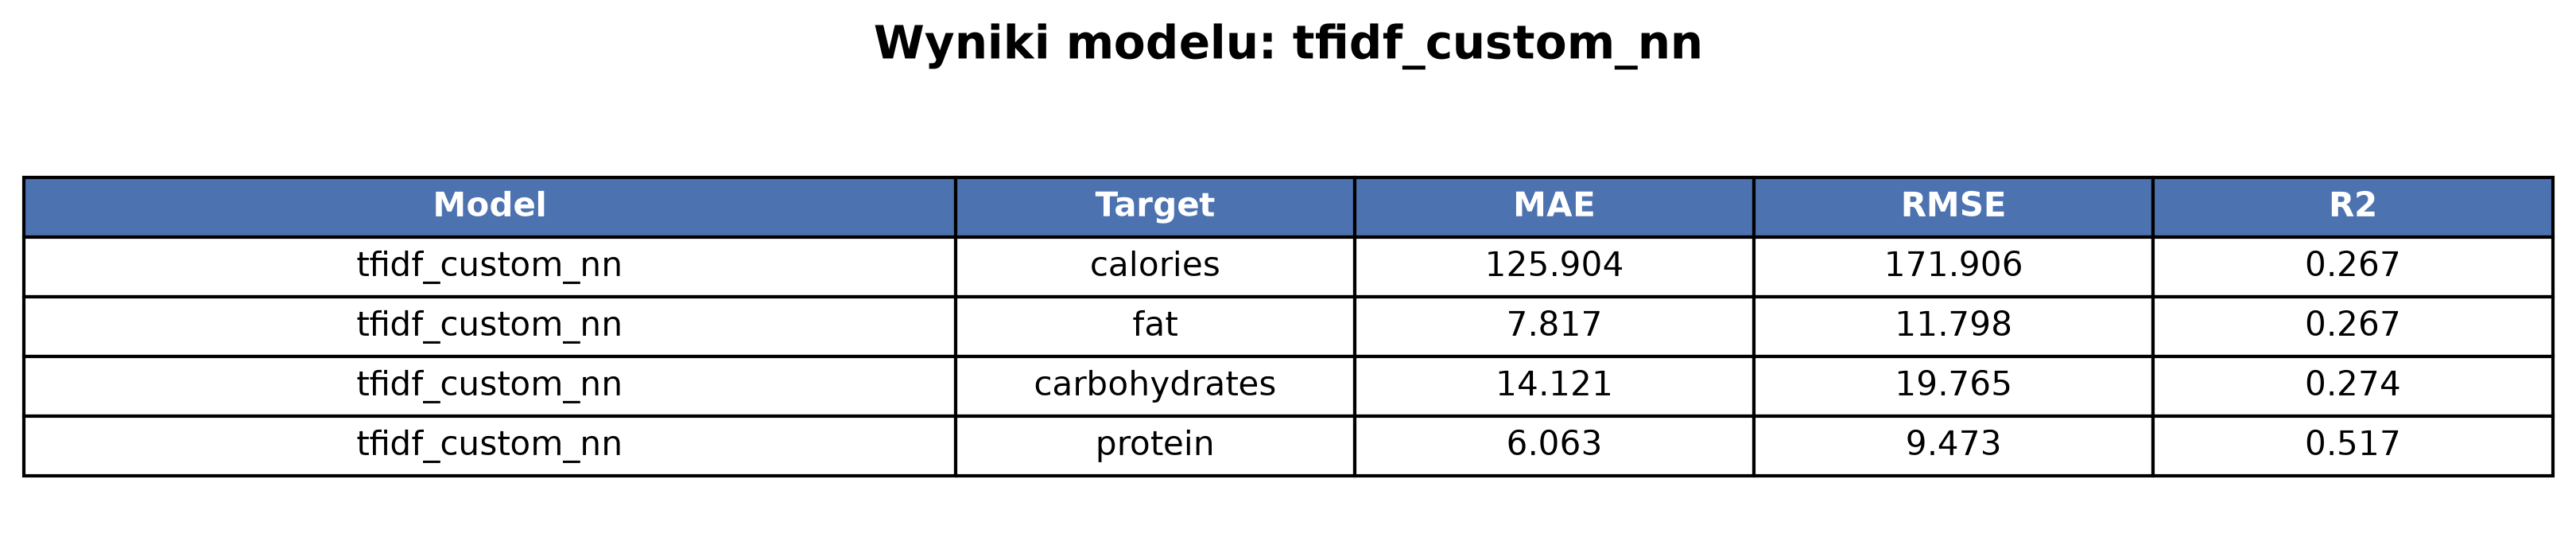
\includegraphics[width=0.8\textwidth]{../img/stats/tfidf_custom_nn.png}
    \vspace{0.5cm}
    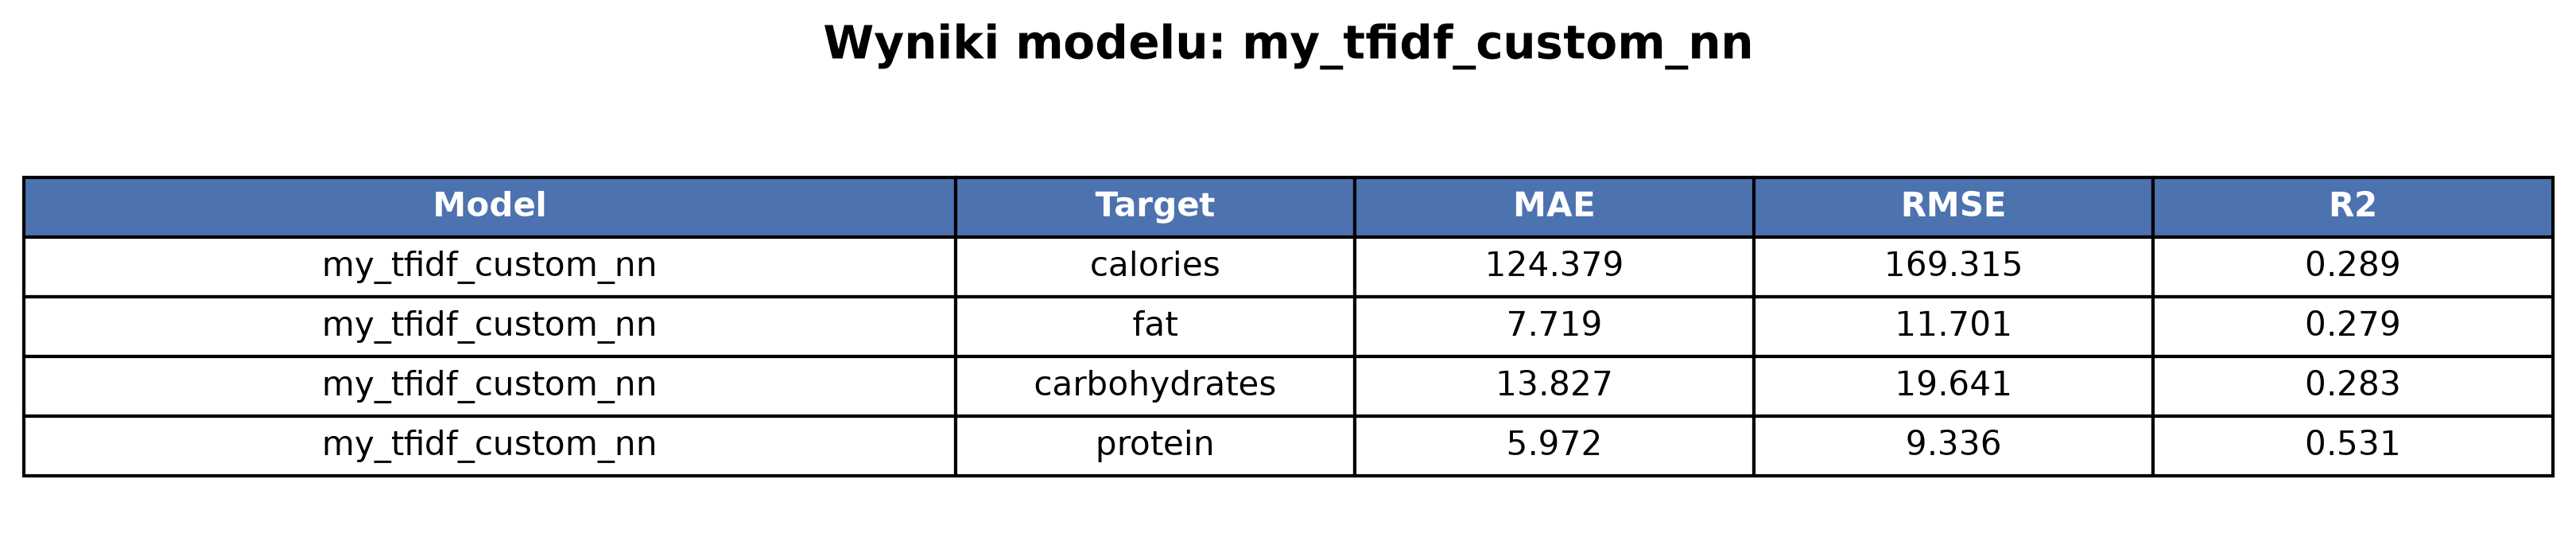
\includegraphics[width=0.8\textwidth]{../img/stats/my_tfidf_custom_nn.png}
    \label{fig:nn_comparison}
\end{figure}
Wyniki są nieco lepsze od naszego modelu regresji liniowej, jednak i tak słabsze od gotowych modeli.
\begin{figure}[H]
    \centering
    \begin{minipage}{0.48\textwidth}
        \centering
        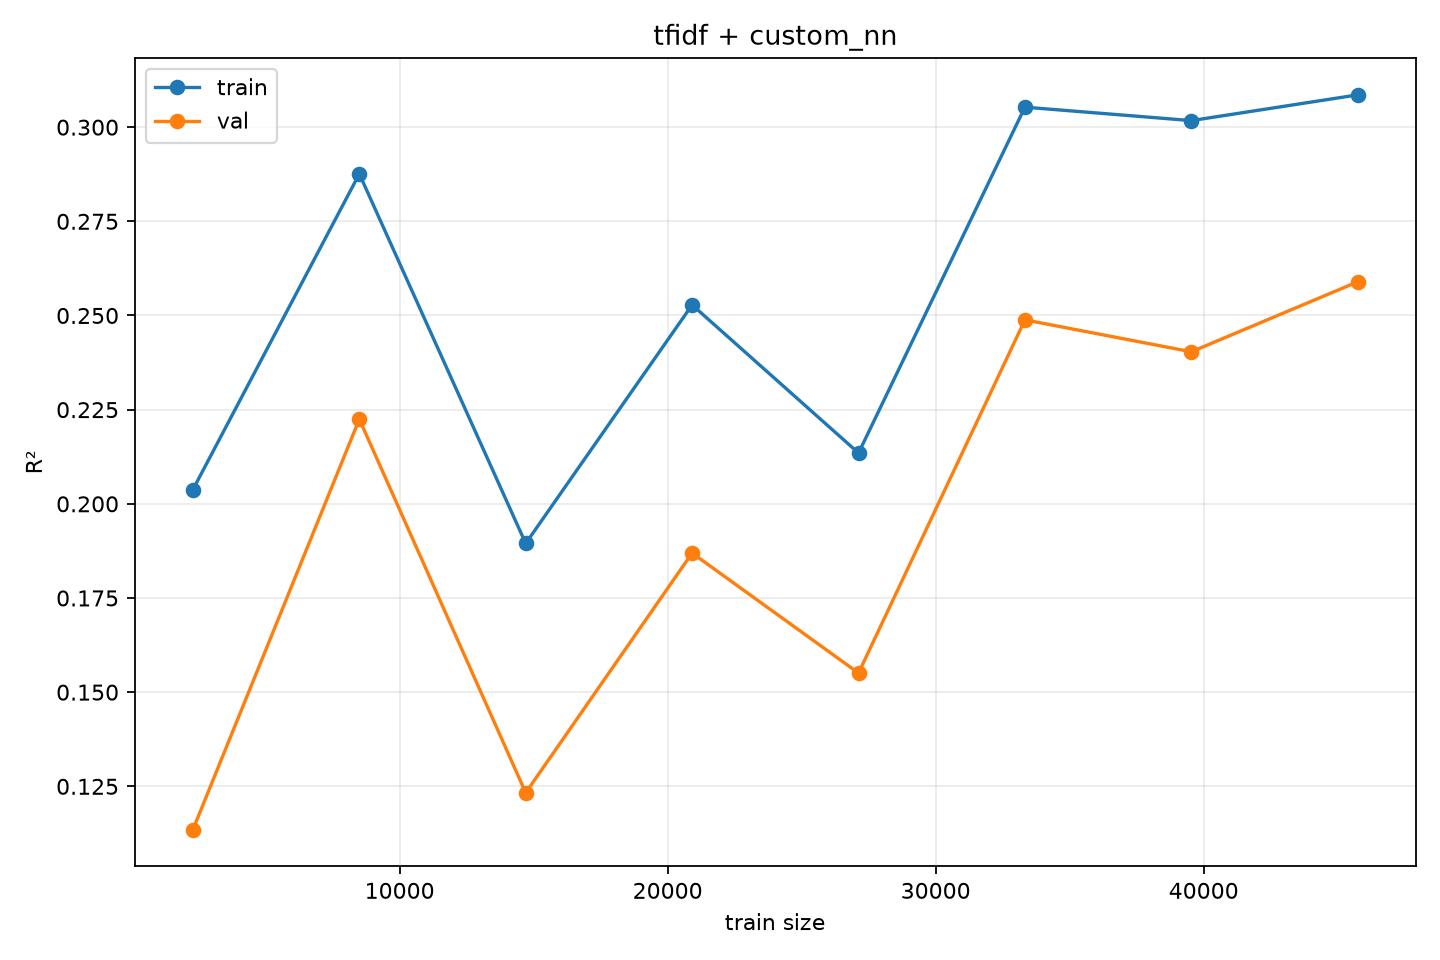
\includegraphics[width=\textwidth]{../img/learning_curve_tfidf__custom_nn2.png}
        \label{fig:learning_curve_nn}
    \end{minipage}
    \hfill
    \begin{minipage}{0.48\textwidth}
        \centering
        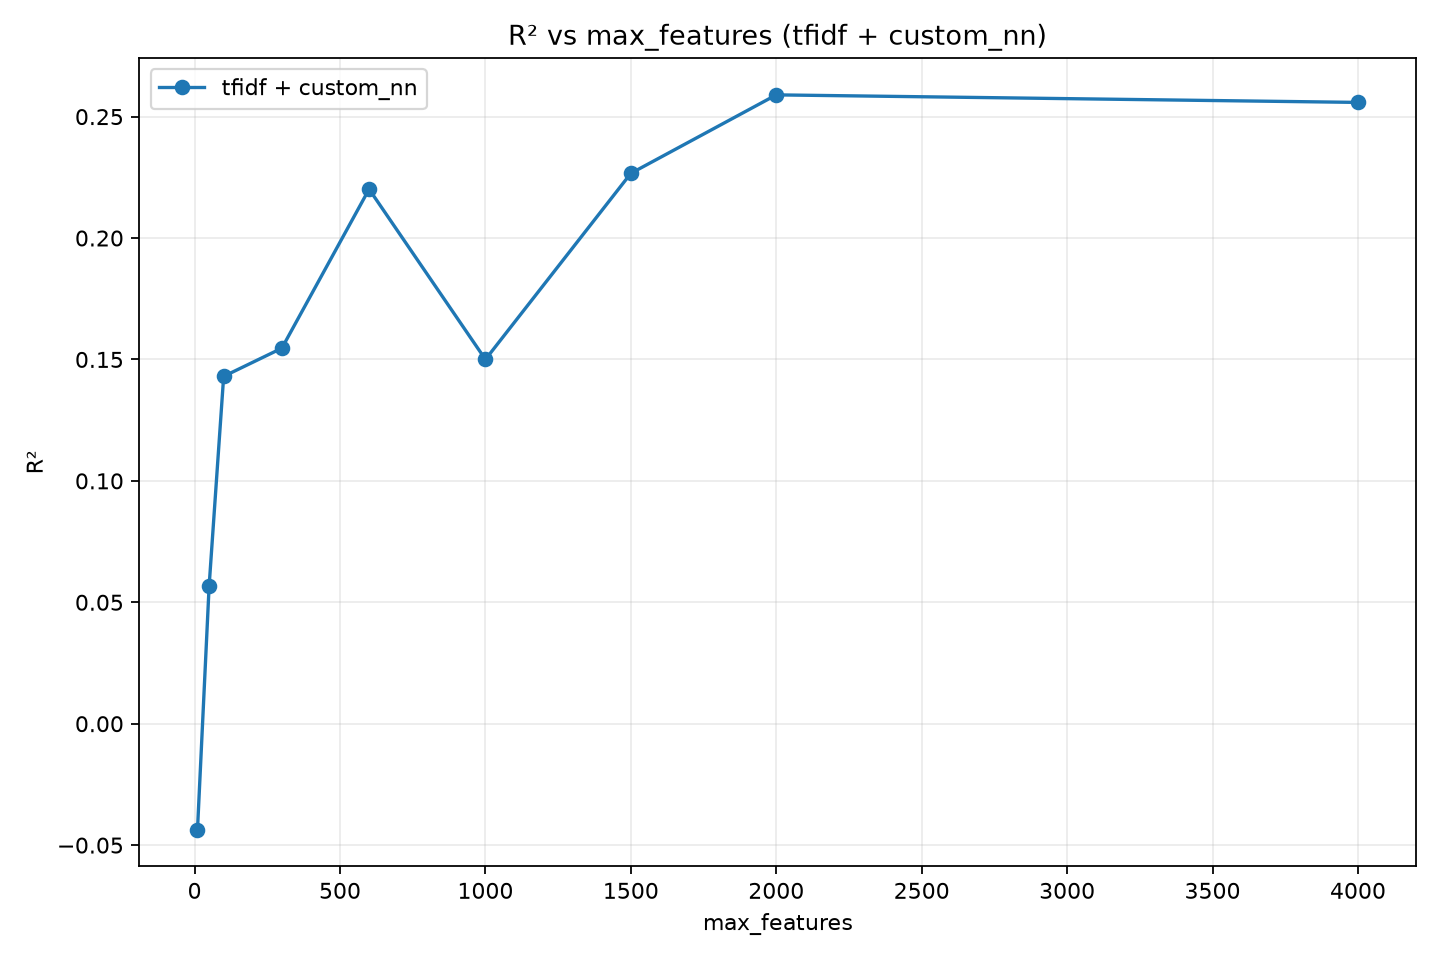
\includegraphics[width=\textwidth]{../img/max_features_tfidf_custom_nn2.png}
        \label{fig:max_features_nn}
    \end{minipage}
\end{figure}

Analizując krzywą uczenia możemy dojść do wniosku, że model wpada w lokalne minima. Próbowaliśmy to naprawić za pomocą optymalizajci adam, jednak nie udało nam się znaleźć parametrów, dla których model zwróciłby dodatnie $R^2$.
Wniosek jest taki, że zdecydownaie można poprawić ten model, ale sam wynik nie jest zły.

\subsection*{Light gradient boosted machine}
Jest to model, który korzysta z boostingu, gdzie jako słabe estymatory wykorzystuje drzewa decyzyjne. Z najważniejszych optymalizaji to ograniczenie nie na głębokość, lecz na liczbę liści w drzewie, dzielenie przedziału wartości ciągłych na bloki w preprocesingu, tak aby rozważać tylko ograniczoną ilość podziałow, pomijanie części obserwacji o małych wartościach gradientu, skupiając się jedynie na wartościach trudnych do sklasyfikowania.\\

W kazdym momencie do drzewa dochodzi dokładnie jeden podział, który najbardziej poprawia wynik, jest to podatne na przeuczenie dlatego mamy stosunkowo niskie ograniczenie na ilość liści. Algorytm korzysta z wielu wątków, podczas rozważania podziałów liści, przez co jest jeszcze szybszy. Dzięki temu mogliśmy wytrenować model z 1000 drzew. Każde drzewo miało 31 liści. 




\begin{figure}[H]
    \centering
    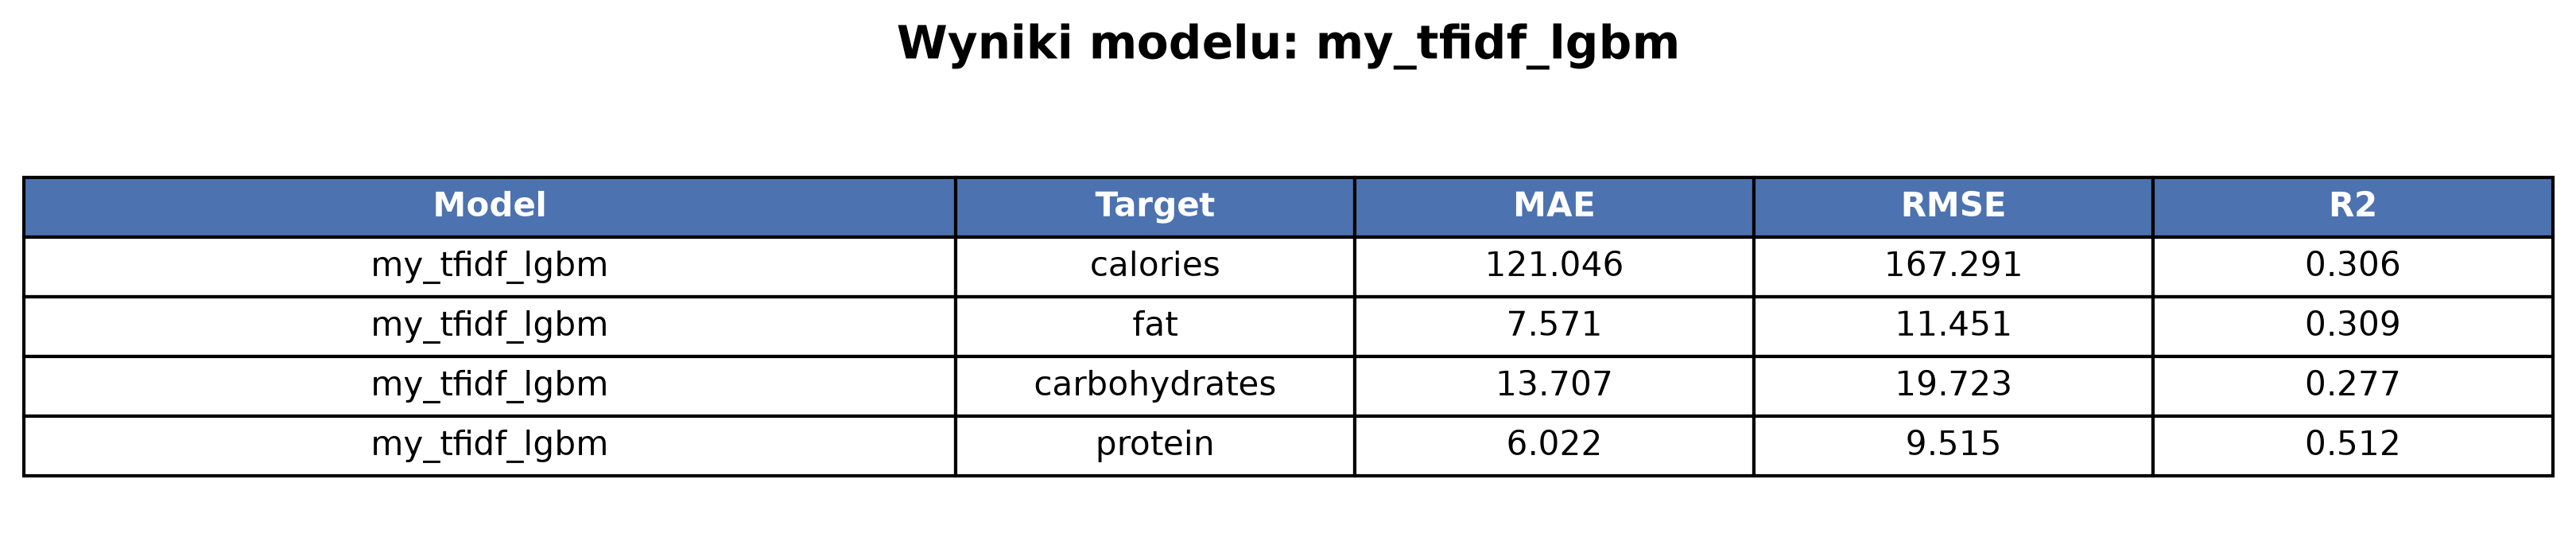
\includegraphics[width=0.8\textwidth]{../img/stats/my_tfidf_lgbm.png}
    \vspace{0.5cm}
    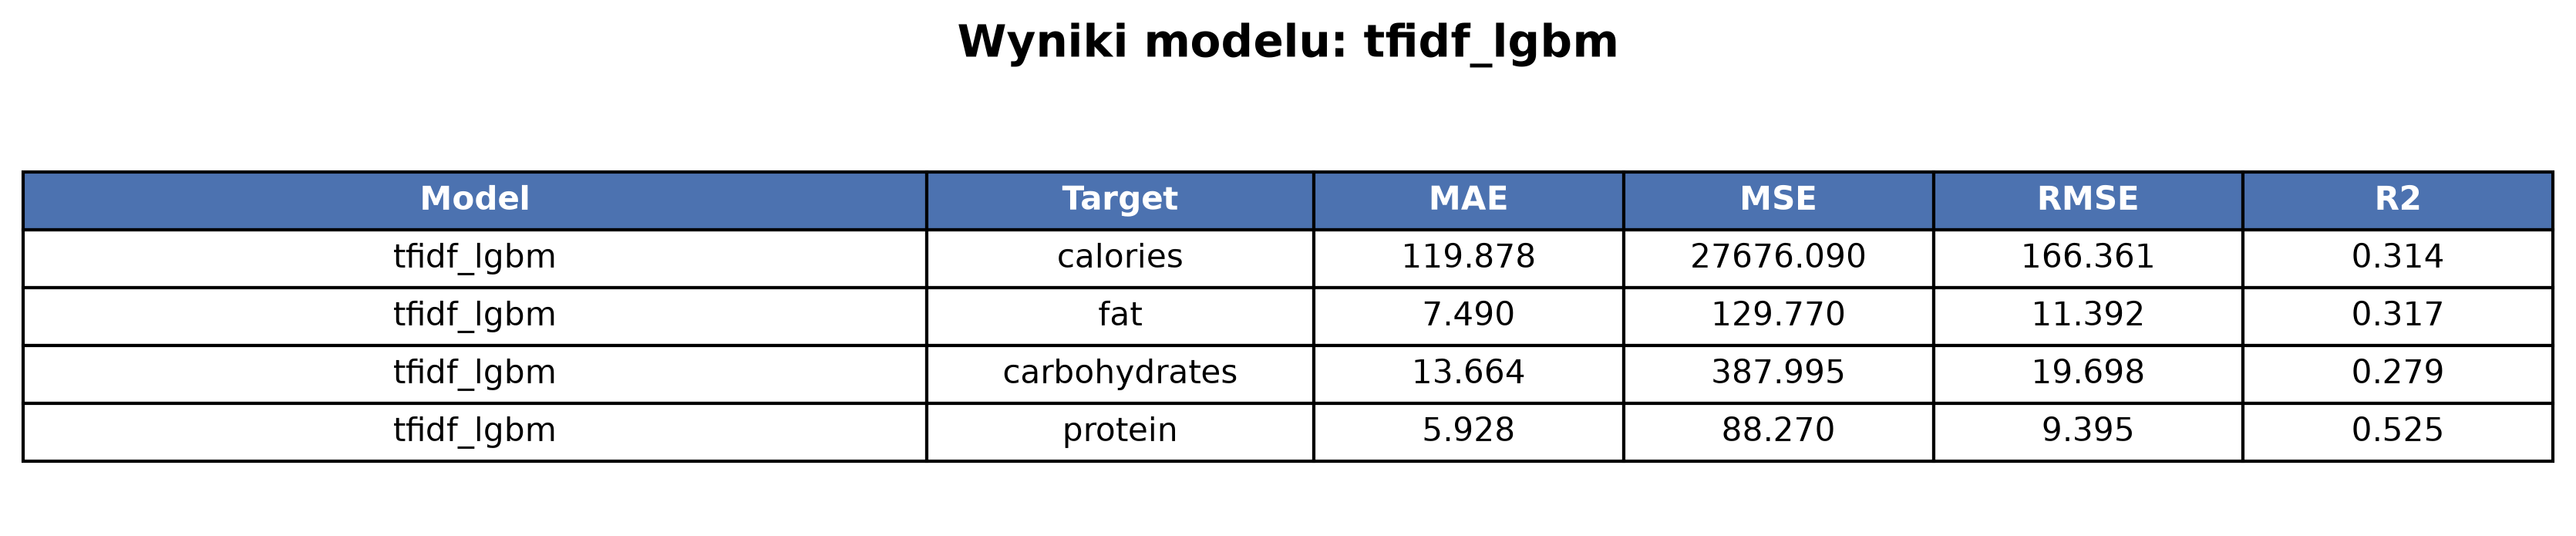
\includegraphics[width=0.8\textwidth]{../img/stats/tfidf_lgbm.png}
    \label{fig:nn_comparison}
\end{figure}
\begin{figure}[H]
    \centering
    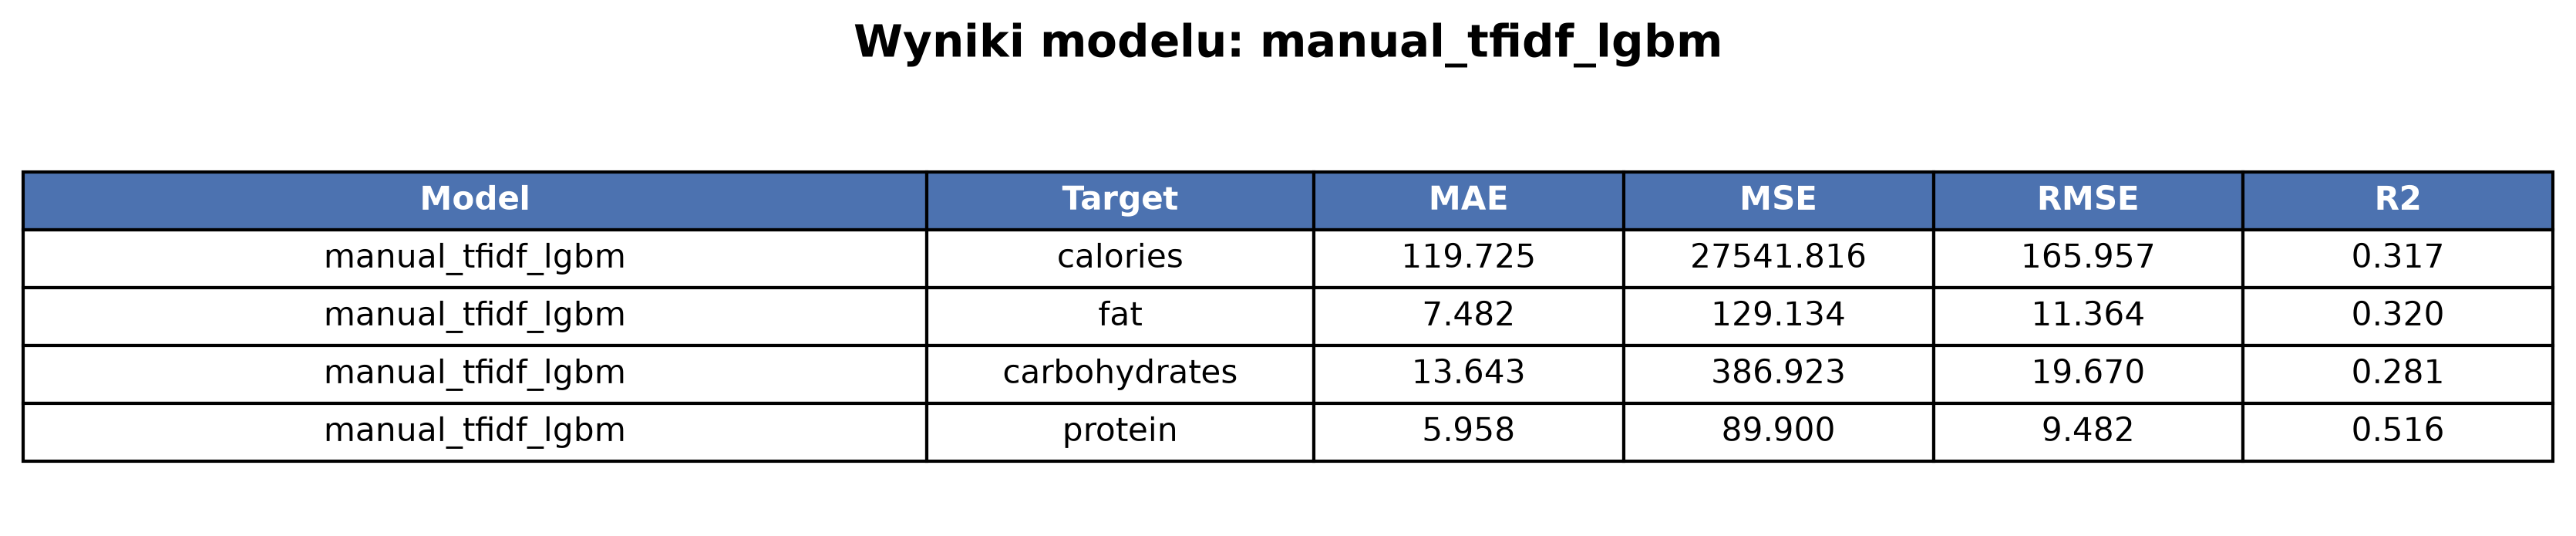
\includegraphics[width=0.8\textwidth]{../img/stats/manual_tfidf_lgbm.png}
    \label{fig:nn_comparison}
\end{figure}
W tym przypadku nasz wektoryzor delikatnie pogarsza wynik, natomiast cechy manualne polepszają. 
\begin{figure}[H]
    \centering
    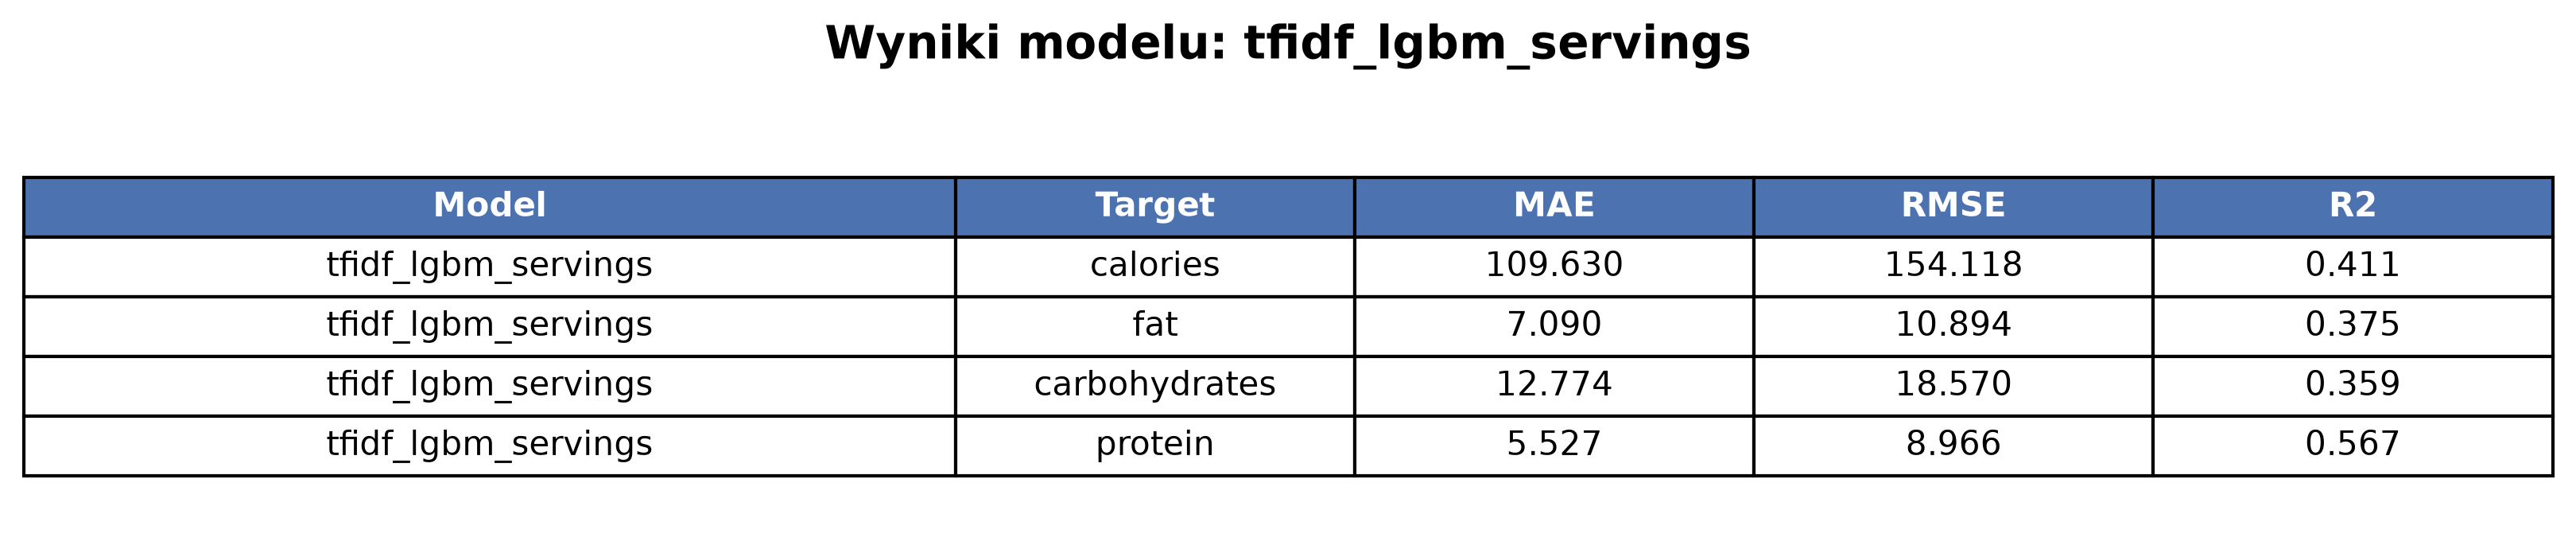
\includegraphics[width=0.8\textwidth]{../img/stats/tfidf_lgbm_servings.png}
    \vspace{0.5cm}
    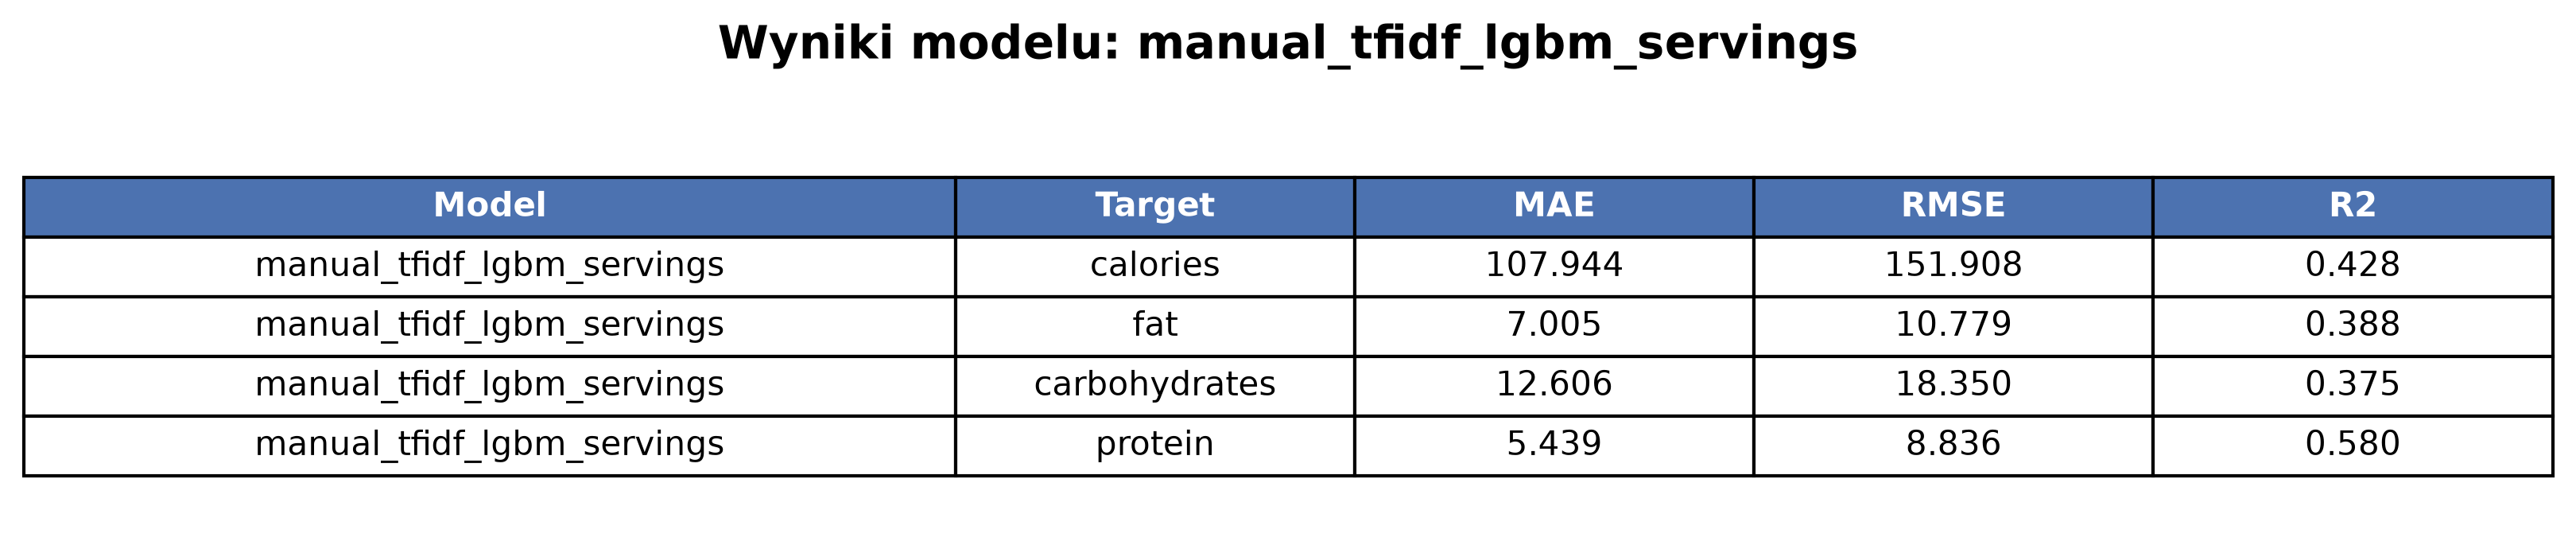
\includegraphics[width=0.8\textwidth]{../img/stats/manual_tfidf_lgbm_servings.png}
    \label{fig:nn_comparison}
\end{figure}

Dodając do tego ilości porcji uzyskujemy najlepszy wynik jaki udało nam się uzyskać. 

\begin{figure}[H]
    \centering
    \begin{minipage}{0.48\textwidth}
        \centering
        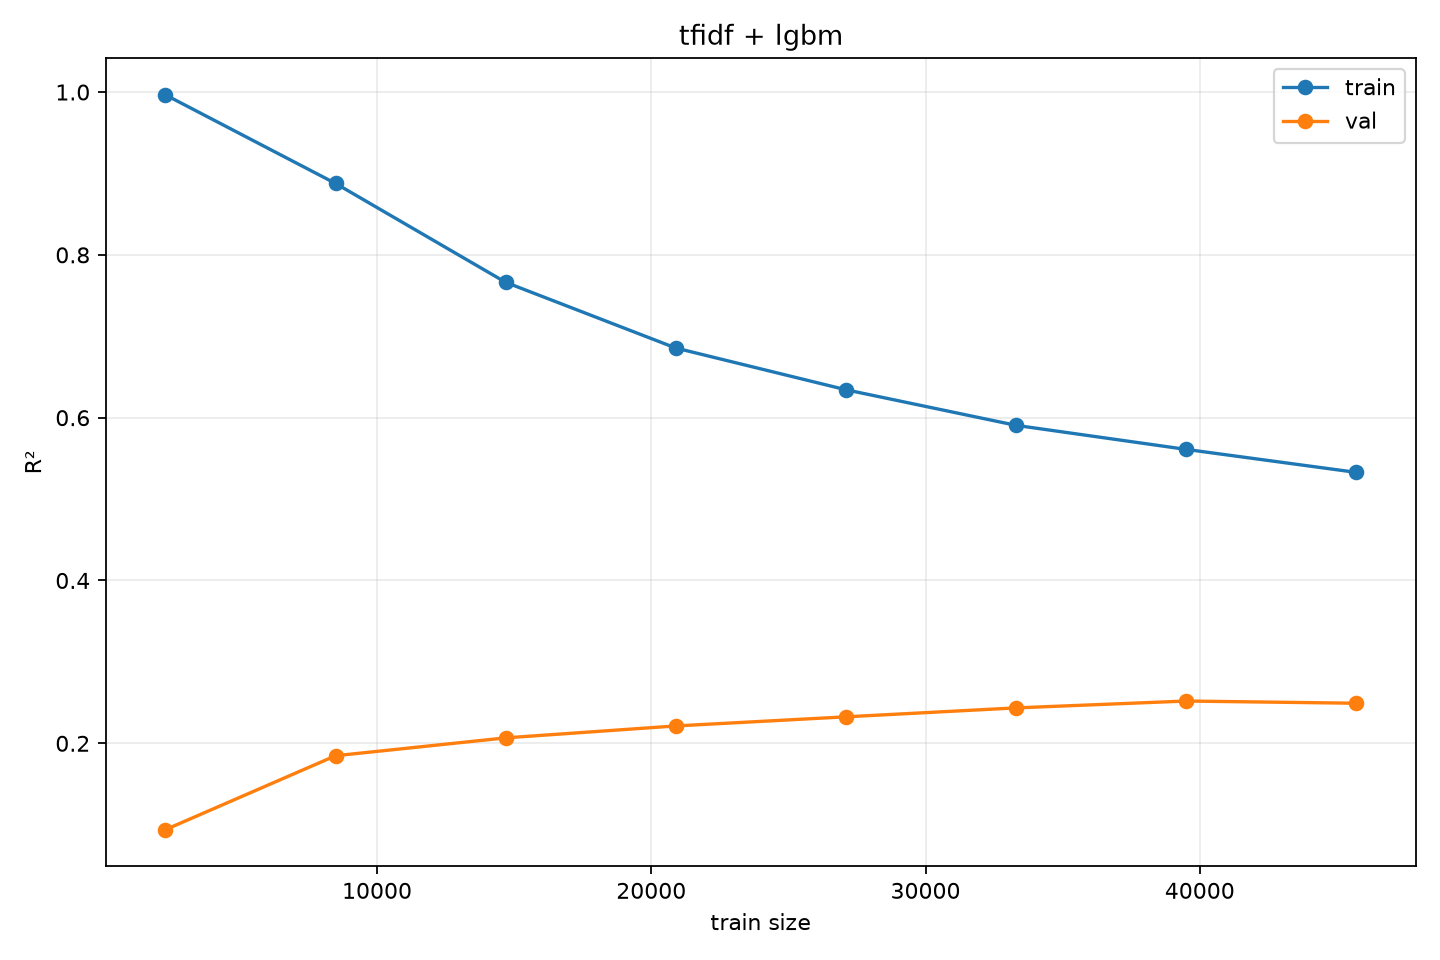
\includegraphics[width=\textwidth]{../img/learning_curve_tfidf__lgbm.png}
        \label{fig:learning_curve_nn}
    \end{minipage}
    \hfill
    \begin{minipage}{0.48\textwidth}
        \centering
        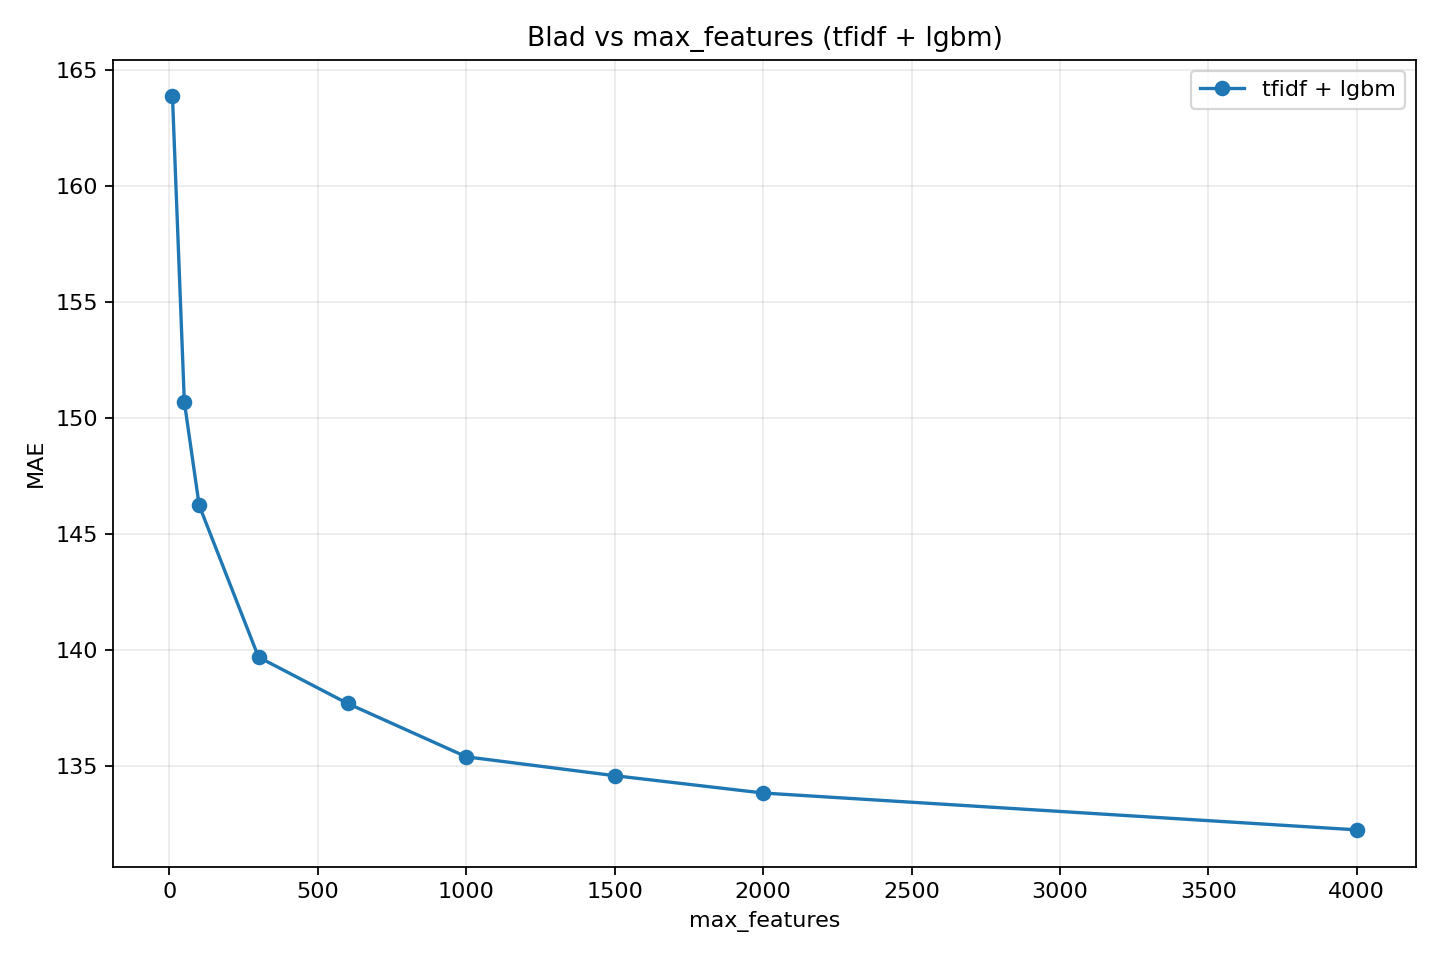
\includegraphics[width=\textwidth]{../img/max_features_tfidf_lgbm.png}
        \label{fig:max_features_nn}
    \end{minipage}
\end{figure}

Analizując krzywą uczenia możemy zobaczyć, że wypłaszcza się ona znacznie wolniej, niż w przypadku krzywej modelu Ridge. Również krzywa ilości cech jest mniej wypłaszczona. Przepuszczalnie wynika to z tego, że model LGBM jest bardziej skomplikowany i uczy się wolniej jednak jest w stanie nauczyć się więcej. Prawdopodbnie przy większych zasobach danych i mocy obliczeniowej byli byśmy w stanie wytrenować go jeszcze lepiej.

\subsection*{Custom AdaBoost Regressor}
Widząc wyniki LGBM, chcieliśmy napisać coś podobnego. Bez tylu optymalizacji, ale żeby było nasze. Udało nam się to napisać z ograniczeniem na liczbę głębokości. Jednak model z grubsza nie działa, a przynajmniej nie działa współpracując z mocą obliczeniową jaką posiadamy. Próbując wytrenować model z 40 drzewami, zajęło to nam prawie 4.5h. A niestety model nic nie przwidywał. Dodanie większej ilości drzew mogło by pomóc, jednak nie byli byśmy w stanie tego wytrenować.
\end{document} 